\documentclass[11pt,letterpaper]{article}
\usepackage[T1]{fontenc}
\usepackage{lmodern,microtype,amsmath,amssymb,amsthm,mathtools,booktabs,array}
\usepackage[letterpaper,top=.92in,bottom=.9in,left=.95in,right=.95in,headheight=15pt]{geometry}
\usepackage{xcolor,fancyhdr,tikz}
\definecolor{ink}{HTML}{142C40}
\definecolor{accent}{HTML}{166861}
\usepackage[unicode,colorlinks=true,urlcolor=accent,linkcolor=accent,citecolor=accent,bookmarksnumbered=true]{hyperref}
\hypersetup{pdftitle={Finite observations in intuitionistic primitive recursive arithmetic},pdfauthor={Research report prepared for Vladimir Reshetnikov}}
\newtheorem{theorem}{Theorem}[section]
\newtheorem{lemma}[theorem]{Lemma}
\newtheorem{proposition}[theorem]{Proposition}
\newtheorem{corollary}[theorem]{Corollary}
\theoremstyle{definition}
\newtheorem{definition}[theorem]{Definition}
\newtheorem{remark}[theorem]{Remark}
\newtheorem{example}[theorem]{Example}
\setcounter{tocdepth}{1}
\setlength{\emergencystretch}{2.5em}
\setlength{\parskip}{2pt}
\pagestyle{fancy}\fancyhf{}
\fancyhead[L]{\small\sffamily\color{ink}Finite observations in iPRA}
\fancyhead[R]{\small\sffamily\color{ink}Research report}
\fancyfoot[C]{\small\sffamily\thepage}
\newcommand{\src}[2]{\href{https://github.com/VladimirReshetnikov/ProveIt/blob/3ee850b4c2d650cf01263823fd5415963747c5d0/Logic/PrimitiveRecursiveArithmetic/#1}{#2}}
\begin{document}
\thispagestyle{plain}
{\noindent\color{accent}\sffamily\small\bfseries FOUNDATIONS OF MATHEMATICS\quad /\quad RESEARCH REPORT}\par\vspace{12pt}
{\noindent\sffamily\bfseries\color{ink}\fontsize{27}{31}\selectfont Finite observations in intuitionistic\\primitive recursive arithmetic\par}
\vspace{7pt}
{\noindent\large Cyclic proofs, exact quotients, and applications to categories, topology, and residues\par}
\vspace{10pt}
{\noindent\small Prepared for Vladimir Reshetnikov\hfill 19 November 2026}\par
\vspace{6pt}\noindent{\color{accent}\rule{\linewidth}{.85pt}}
\begin{abstract}
We prove a quantitative extension theorem for maps on regular names, and give a finite interpretation for mathematical assertions whose observable content can be generated by mutually dependent positive rules. A bounded iteration constructs both a proof for every reachable assertion and a checkable obstruction for every unreachable one. We characterize exactly which identifications of data preserve every transition and compute the coarsest admissible refinement of a proposed identification. We then give three applications of finite presentations: a decision and separating diagram for final functors, geometric and homological nerve theorems with explicit contraction algorithms, and a residue formula at primitive-recursively named complex centres. A square-root monodromy calculation illustrates all three viewpoints on one finite graph. The arithmetic proofs use fixed primitive recursive programs, finite encodings and quantifier-free induction. We identify the object derivations checked in Lean, the native Lean results, and the analytic premises used from earlier human proofs.
\end{abstract}
\tableofcontents
\newpage
\section{What is being interpreted?}\label{sec:meaning}
A functor on a finite category can be given by tables. A holomorphic function on an annulus generally cannot. A proof about the latter can still use a table at each requested accuracy, provided that a specified program produces the table and another argument justifies its use. Confusing these two obligations loses exactly the hypotheses on which the analytic theorem depends.

We use the repository's ordinary iPRA: intuitionistic first-order logic with equality, successor axioms, the equations of all primitive recursive (PR) symbols, and induction for quantifier-free formulas with parameters. The following are three readings of variables used throughout.
\begin{enumerate}
\item A graph, finite category, matrix, precision or rational polygon is a number in the object theory. A theorem uniform in these inputs has numerical quantifiers.
\item An evaluator such as $A(j,n)$ is fixed PR syntax outside the object theory. Its numerical arguments remain arbitrary inside the theorem. Different fixed evaluators give a schema; a single family with a uniform evaluator may carry an additional numerical index. The ring of Gaussian rationals is denoted by $\mathbb Q(i)$.
\item A completed object is interpreted through its stipulated names and observations. Statements about all represented functions abbreviate families of first-order implications from their contracts. Statements about all classical functions would require a separate adequacy theorem for that source language.
\end{enumerate}
An elementary diagonal argument explains the distinction in the second item. If a total PR function $E(e,x)$ evaluated every unary PR program for some index $e$, then $x\mapsto E(x,x)+1$ would have an index $d$, giving $E(d,d)=E(d,d)+1$. Supplying finite tables or a fixed evaluator avoids this universal evaluation assumption.

\paragraph{Arithmetic conventions.}
For a list of $l$ entries below $B$, take the pair of $l$ and a base-$\max(2,B)$ word, with the first entry the least significant digit. Store numerical bounds separately when needed. Take, for example, the injective pair $2^a(2b+1)$ with a reserved value $0$. For positive inputs its projections are obtained by counting divisions by two up to the input. Totalize exceptional divisions and invalid projections to zero, and test validity before using their equations. Signed integers can be given by a sign and magnitude and rationals by a signed numerator and a positive denominator. Order and equality are checked by multiplication, including for noncanonical fractions. Maxima over empty numerical lists are zero. Bounded Boolean conjunction, disjunction, sum, minimum with a sentinel, table lookup and replacement are PR. Binary vectors of length $N$ are integers below $2^N$.

For a fixed bounded numerical formula its truth bit can be proved equivalent to the formula in iPRA. For example, for a bounded disjunction scan indices while recording a bit and the first successful index; induction on the scan proves that the bit is one exactly when a witness is present. Negation and implication on decidable bits have their Boolean truth tables intuitionistically. Use this construction recursively on the fixed formula, or apply the repository's \src{Derivations/Lean/IPRADerivations/Foundations/BoundedSyntax.lean}{bounded-syntax compiler}. In particular a bounded conjunction of invariants at a variable number of addresses is a single quantifier-free bit equation for induction. An outer universal parameter can be fixed before the induction when the step preserves that parameter.

\paragraph{An observation and its obligations.}
In the most general interface used here an input presentation $p$, an observation request $q$, an answer $u$ and evidence $e$ have a fixed PR verifier $V(p,q,u,e)$. The client states what a successful check implies in its chosen interpretation. A solver additionally gives a PR producer with a proof of success under its explicitly stated input hypotheses. To pass from named inputs to intrinsic conclusions it must also prove invariance: two admissible presentations of the same input give equivalent observations at the promised accuracy. For example, equality of name samples at one index rarely suffices, while an exact path parity can be invariant under every change of local square-root signs. Composition discharges the next operation's input checks with the previous operation's output proofs. A modulus is used where that next check requires a more accurate sample. No unrestricted choice of witnesses enters this procedure.

\subsection{Continuous maps from rational observations}\label{sec:completion}
A useful connection between the finite and analytic parts is the universal property of completion in its quantitative form. A presentation $X$ here has decidable valid codes, a PR rational pseudometric $d_X$ on them, and proofs of its laws. A constant name is the constant sequence at a valid code. With $e_n=2^{-n}$, the distance assertion on names is the first-order formula
\[
 B_X(r;a,b):\qquad \forall i,j\quad d_X(a_i,b_j)\le r+e_i+e_j .
\]
The programs $a,b$ are externally fixed; $i,j$ are numerical variables. A regular name has $B_X(0;a,a)$ and valid values. Equivalent names satisfy $B_X(0;a,b)$. The triangle inequality holds for this notation: compare across the common intermediate sample $c_h$ and then remove the excess $2e_h$. For rational quantities this removal is constructive. If the proposed inequality of rationals failed, its positive gap would exceed $2e_h$ at an index calculable from a positive denominator. Thus agreement is an equivalence relation on regular names.

Let a rational-input evaluator $E(x,i)$ produce valid $Y$-codes, with a PR modulus $\mu$. Assume that for all valid $x,y$ and all numerical $k,i,j$,
\begin{equation}\label{eq:approx}
 d_X(x,y)\le e_{\mu(k)}
 \quad\Longrightarrow\quad
 d_Y(E(x,i),E(y,j))\le e_i+e_k+e_j .
\end{equation}
This single condition includes regularity at fixed $x$ by letting $k$ increase with $y=x$.

\begin{theorem}[Uniform extension and composition]\label{th:completion}
Define $s(n)=\max(n+2,\mu(n+2)+1)$ and
$\widehat E(a)_n=E(a_{s(n)},n+2)$. It gives a regular name, depends only on the equivalence class of $a$, and extends $E$ on constant names. It sends $B_X(e_{\mu(k)+1})$ to $B_Y(e_k)$. Among extensions with supplied uniform moduli it is unique up to equivalence of output names. Two such extensions compose by PR substitution.
\end{theorem}
\begin{proof}
For equivalent inputs $a,b$, fix output indices $n,m$. Compare the two outputs through $E(a_L,j)$ with $L=\max(s(n),s(m))$ and $j=\max(n+2,m+2)$. The regularity of $a$ gives $d_X(a_{s(n)},a_L)\le2e_{s(n)}\le e_{\mu(n+2)}$. The analogous inequality $d_X(a_L,b_{s(m)})\le2e_{s(m)}$ follows from equivalence. Two applications of (\ref{eq:approx}) give a total distance at most $2e_{n+2}+2e_{m+2}+2e_j\le e_n+e_m$. This proves both regularity and presentation independence. A constant name gives samples $E(x,n+2)$, equivalent to $E(x,n)$ by fixed-input regularity.

For the modulus, suppose $B_X(e_{\mu(k)+1};a,b)$. At a large common index $L$ take $2e_L\le e_{\mu(k)+1}$, so $d_X(a_L,b_L)\le e_{\mu(k)}$. For fixed $n,m$ also require $L\ge s(n),s(m)$. Compare the two output samples through $E(a_L,j)$ and $E(b_L,j)$. The two outer errors cost $2e_{n+2}+2e_{m+2}+2e_j$ by the preceding calculation applied on each input separately. The middle error costs $e_k+2e_j$. For arbitrarily large $j$ this gives the desired $e_n+e_k+e_m$ bound. All sufficiently large indices here have explicit lower bounds.

The constant name at $a_L$ is within $B_X(e_L)$ of $a$. If another extension has a modulus, choose $L$ large enough to obtain output tolerance $e_k$ for each extension at this pair of inputs. Their outputs agree on the constant by hypothesis. The ball triangle inequality puts their outputs at $a$ within $B_Y(2e_k)$ for every $k$, hence they are equivalent. Finally, for $F:Y\to Z$ in this sense, use the rational-input name $G(x,n)=\widehat F(E(x,\cdot))_n$. If $d_X(x,y)\le e_{\mu_E(\mu_F(k)+1)}$, (\ref{eq:approx}) gives $B_Y(e_{\mu_F(k)+1};E(x,\cdot),E(y,\cdot))$, so the modulus just proved gives $B_Z(e_k)$ for the two $G$-names. This supplies (\ref{eq:approx}) for $G$. The composite on arbitrary names is uniformly continuous and agrees with $G$ on constants, so uniqueness gives the composition law. The identity evaluator $E(x,i)=x$ yields the identity on names by the same argument.
\end{proof}

The theorem gives a common interface for a rational piecewise-linear map, a chart evaluator, and their composites. It also specifies what must be added on a restricted domain: the sampled codes must stay in the region on which (\ref{eq:approx}) is proved. The positive annular collar in Section~\ref{sec:named-residue} furnishes precisely this input for translation. A global compactness principle is unnecessary for the extension once the modulus is supplied.


\section{Cyclic systems of finite observations}\label{sec:closure}
The \src{Derivations/FIBER-CLAIMS.md}{FIBER audit} distinguishes closure of precision demands from execution of mutually dependent certificate producers. An inequality specifying how much data to request does not produce evidence for either of two rules which call each other. We handle a precisely delimited case of cyclic execution: all relevant states, evidence values and local rule instances can be grounded in PR-bounded finite sets, and previously established facts occur positively. This includes cyclic systems with several simultaneous premises and several possible producers of the same conclusion.

\begin{definition}
Fix a numerical input $p$ (including the observation request if needed). The ground atoms are $[N]=\{0,\ldots,N-1\}$. Rules $i<M$ consist of a head $h_i<N$ and a bit mask $B_i\subseteq[N]$. Read $B_i\Rightarrow h_i$ as a production. A rule with empty body is a seed. A local decidable guard can delete a rule. For a schema, $N,M,h_i,B_i$ and the guard are fixed PR functions of their numerical inputs. A property tested negatively in the guard must already be decidable from the input.
\end{definition}
Addresses can contain a tag, a request and its answer payload. To ground a producer depending on its predecessors' actual evidence, enumerate allowed tuples of predecessor addresses and evidence in their supplied finite bounds, run the guard, and put exactly the matched tuple in the body. If two premises must use the same witness, one tuple must encode that agreement. Unrelated existential facts at two addresses do not guarantee compatible witnesses.

Define the inflationary operator and its layers by
\[
 T(X)=X\cup\{h_i:B_i\subseteq X\},\qquad X_0=\varnothing,\qquad X_{j+1}=T(X_j).
\]
The producer reads a frozen copy of $X_j$ throughout round $j+1$. A certificate for $a$ is a list of at most $N$ distinct addresses ending in $a$, each with a rule for its head whose premises occur earlier. A \emph{cut} for $a$ is a mask $C$ with $a\notin C$ and $B_i\subseteq C\Rightarrow h_i\in C$ for every rule. These definitions include $M=0$ and $N=0$; requests for a particular atom require $a<N$.

\begin{theorem}[Production or obstruction]\label{th:closure}
After $N$ rounds the layer $L=X_N$ is the least closed mask. A PR algorithm produces, for each $a<N$, either a certificate for $a$ or a cut for $a$. No atom admits both. Under any assignment of iPRA formulas $P_a$ and any context $\Gamma$, local derivations taking the $P_b$ for $b\in B_i$ to $P_{h_i}$ over $\Gamma$ replay each positive certificate as a derivation of $\Gamma\vdash P_a$.
\end{theorem}
\begin{proof}
Every step preserves old bits. If it changes a mask, the first new bit exists by bounded search, and counting the bits gives an increase of at least one. If it leaves a mask fixed, all subsequent masks are equal to it by the defining equation of iteration. More precisely, at each $j$, either $T(X_j)=X_j$ or $j\le |X_j|$. The base is immediate. In the nonstationary case use the strict increase to carry the inequality forward; in the stationary case substitute the fixed mask at the next step. Since a subset of $[N]$ of size $N$ is the whole set, $X_N$ is stationary. If $C$ is closed, $X_0\subseteq C$ and $X_j\subseteq C$ implies $T(X_j)\subseteq C$ by checking every firing rule. Induction with $C$ fixed gives leastness.

For each new bit store its round and the first enabling rule. Sort the addresses by (round,address); for a requested $a$ keep its backward dependencies, or just take the prefix ending in $a$. Every premise has a strictly smaller round. Pointers may be reused at multiple heads. A cut certificate for an absent bit is $L$ itself. A scan of any positive certificate shows its entries belong to every closed $C$, proving incompatibility. Replay the positive list in order, using the local derivation at each line and simultaneous cut on previously obtained derivations. Induction in this last assertion is in the metatheory on a particular finite derivation; it introduces no object-theory induction for arbitrary $P_a$.
\end{proof}

The list has at most $N$ pairs with entries below, for instance, $1+N(M+1)$. Its word bound is $\max(2,1+N(M+1))^N$. Invalid rules or addresses can be rejected by a bounded precheck. A table of birth rounds and rule numbers fits in the same type of coding, with base $2+(N+1)(M+1)$. The report's cardinality proof uses the bit equation for the dichotomy and the bounded sum of bits. Thus the proof for numerical inputs has only quantifier-free inductions once the bounded predicates are compiled. A rank for a one-line self-call with no seed is never manufactured. The empty mask is a cut excluding that head when this is the only rule.

\paragraph{Source meaning and completeness.}
If every production has been justified, acceptance suffices for its source observation. A cut only excludes proof by these productions. To interpret rejection as mathematical impossibility one needs a converse: every source witness can be converted to a finite production proof in the chosen finite model. In the monodromy example a path gives such a proof by reading its edges; for an unconstrained existence theorem a converse may fail. If grounding uses a subgraph of a larger presentation, negative certificates extend when \emph{all} rules with a retained head are covered, with their bodies in the retained subgraph (or with verified summaries for discarded premises). Restrict any global proof down its branches to see this. Dropping incoming rules from outside a chosen precision budget generally loses completeness.

\subsection{When may two addresses be identified?}\label{sec:quotient}
Payloads often dominate the number of ground states. The following test computes the coarsest refinement of a proposed identification that preserves \emph{one-step behaviour on every union of classes}. The extra universal condition permits reuse of the same quotient with arbitrary blockwise initial data.

Let $P$ be a partition of $[N]$ and $[a]_P$ its block. For head $a$ collect the finite family
\[
 D_P(a)=\{\{[a]_P\}\}\cup
   \bigl\{\{[b]_P:b\in B_i\}: h_i=a\bigr\}.
\]
Discard duplicate sets and proper supersets of another member, leaving an antichain $S_P(a)$. The first singleton records persistence. A seed gives the empty set and dominates every other term. A partition is \emph{stable} when $T$ sends every union of its blocks to a union of its blocks.

\begin{theorem}[Coarsest stable refinement]\label{th:quot}
A partition is stable exactly when $S_P(a)=S_P(b)$ for every pair in a common block. Split every block by this signature and repeat up to $N$ times. The resulting partition is the unique coarsest stable refinement of the starting partition, up to block names. Its quotient iteration lifts exactly at every round for every blockwise initial mask. Each split has a finite counterexample to stability at that stage.
\end{theorem}
\begin{proof}
For a set $U$ of blocks write $\widehat U$ for their union. By the rule equation,
$a\in T(\widehat U)$ iff some $D\in D_P(a)$ is contained in $U$, equivalently some minimal member is. The Boolean implication from the family for $a$ to that for $b$ on all $U$ holds iff every term $D$ for $a$ contains some term for $b$: necessity follows by setting $U=D$, and sufficiency by inclusion. Mutual implication of two finite antichains forces equality: given $D$ on the first side choose $E\subseteq D$ on the second and $D'\subseteq E$ on the first. Minimality gives $D'=E=D$. A failure of one implication supplies a specific $U=D$ witnessing a split.

A proper refinement increases the number of nonempty blocks, bounded by $N$. If a round is unchanged its signature test succeeded. Hence $N$ rounds suffice, including the empty partition. Let $Q$ be any stable refinement of the original partition. If $Q$ refines the current $P$, any $P$-block union is a $Q$-block union. Equal $Q$-colours then have identical next-step bits on it. By the signature criterion they survive the next split together. Induction shows $Q$ refines the eventual result, proving the asserted universal property. For a stable $P$ put one rule per signature member on its quotient, with that block as head. The defining test gives $\widehat{\overline T(U)}=T(\widehat U)$, whence equality at every round by induction.
\end{proof}
Choose each block's least address as its name. Every family has at most $M+1$ input terms per head and every term fits in $N$ bits. Pairwise subset tests and a scan over heads suffice for each refinement, with no search over partitions. One may avoid even explicit antichains by the mutual implication test in the proof. These loops with the $N$-round cap give a PR refinement algorithm. Eager reachability from the empty set alone can permit coarser identifications: the universal property specifies exactly what this stronger test computes.

\paragraph{A failed quotient.}
Take six atoms $P_0,P_1,Q_0,Q_1,R_0,R_1$; seed $P_0,Q_1$ and add $P_i,Q_i\Rightarrow R_i$ for $i=0,1$. Forgetting $i$ in all three pairs gives a false derivation of $R$. The original least mask is $\{P_0,Q_1\}$. The first refinement separates the seeded and unseeded $P$ and $Q$ addresses. The next separates the two $R$ addresses, since their premises now use different blocks. This is the loss of a shared witness in a join that shares an index; the procedure detects it before the quotient is used as a proof.

\paragraph{Use across the applications.}
Connectivity predicates for a comma category, path classes in a diagram quotient, and compatible choices of a sheet on an edge are finite rule systems directly. In the nerve construction the larger objects are finite chain matrices; a linear solve produces the witnesses needed by transfer rules. In the residue construction infinitely many observations are handled one request at a time. Chart estimates translate the precision request into finitely many local computations and justify the transfer of their answers. The analytic argument does not rely on treating all holomorphic functions as a finite collection of states.

\section{Deciding when a change of index preserves every finite colimit}
\label{sec:effective-finality}

Consider a calculation assembled from local finite sets, with specified maps between them. One would like to drop or duplicate some indexing objects without changing the result of gluing. A change of index can work for one particular diagram by accident. We give a uniformly primitive recursive test which answers the question for \emph{every} finite-set-valued diagram of the given shape. A negative answer supplies the diagram on which the comparison fails. The ordinary categorical criterion is the final-functor theorem (also called cofinality, Stacks Project, \href{https://stacks.math.columbia.edu/tag/09WN}{Tag 09WN}). Its uniform arithmetic content depends on how quotients, paths, and obstructions are represented.

The repository's \texttt{ipra\_categorical\_methods} develops finite diagram colimits by graph connectivity. The object-calculus module \texttt{Foundations/FiniteCoequalizer.lean} instead merges two labels per generating pair. Its header explicitly leaves identification of the fibres with the generated equivalence, compact indexing of classes, and the general diagram reduction untreated. We give a bounded proof for that very merge algorithm, then use the completed quotient in the index-change test.

\subsection{A quotient with paths and contiguous class numbers}

Write $[n]=\{0,\ldots,n-1\}$. Take a graph on $[N]$ with a list of $m$ oriented edges $(a_i,b_i)$. A zigzag is a vertex followed by a list of edge indices with a direction bit. The checker follows the indicated endpoints and verifies the final vertex. An edge may be traversed in either direction. Initialize $L_0(x)=x$. At step $i$, put $A=L_i(a_i)$ and $B=L_i(b_i)$ and replace each occurrence of $B$ by $A$ in the old label table. Denote the result by $L_{i+1}$. This is simultaneous replacement using the old $A,B$.

\begin{lemma}[Exact fibres of the sequential merge]
\label{lem:label-exact}
$L_m(x)=L_m(y)$ if and only if a zigzag joins $x$ and $y$. A PR function of the graph and the pair returns such a zigzag whenever the labels agree. Every label is a fixed point. The quotient can be numbered as $[r]$ with a PR section.
\end{lemma}
\begin{proof}
Keep a path $p_i(x)$ from $x$ to $L_i(x)$, initially empty. If $L_i(x)\ne B$, keep the path. Otherwise follow $p_i(x)$, then $p_i(b_i)$ in reverse, then the new edge from $b_i$ back to $a_i$, then $p_i(a_i)$. These endpoints match by the update condition. If all old paths have length at most $H_i$, the new bound is $H_{i+1}=3H_i+1$ with $H_0=0$. Thus $H_i=(3^i-1)/2$. This deliberately loose clock avoids a termination argument about shortest paths. The path tables and labels can be updated together by primitive recursion. For instance, lists of at most $2H_m$ signed edge indices are coded by length and fixed-width digits in base $2m+2$. Verification of all $N$ stored paths is a bounded test.

After step $i$ the endpoints of every edge already processed have equal labels. For the new edge both labels become $A$. For each previous edge apply the same replacement function to its two equal labels. The invariant is a bounded conjunction over the first $i$ edges. Consequently the final labels agree along any supplied zigzag, by induction over its successive vertices with its code fixed. Conversely, if the labels of $x$ and $y$ agree, concatenate $p_m(x)$ with the reverse of $p_m(y)$. This gives a path of length at most $2H_m$. Applying the forward implication to $p_m(x)$ gives $L_m(x)=L_m(L_m(x))$.

List in increasing order precisely the $v<N$ satisfying $L_m(v)=v$, say $s_0,\ldots,s_{r-1}$. Set $q(x)=\#\{v<L_m(x):L_m(v)=v\}$. The preceding fixed-point identity gives $s_{q(x)}=L_m(x)$, and counting the preceding list entries gives $q(s_k)=k$. A table $t:[N]\to[z]$ equal on the generating edges is constant along each supplied path; its unique factor is $k\mapsto t(s_k)$. The factor equation uses $p_m(x)$ and uniqueness follows by evaluating at $s_k$. If $N=0$ valid input forces $m=0$, and $r=0$ with empty structure maps. No positive-base digit operation is required in this case.
\end{proof}

A finite category $K$ has object and arrow lists, source and target tables, an identity table, and a composition table on composable pairs. The typing, identity and associativity checks scan at most triples of arrows. A finite-set diagram $D$ assigns $[n_d]$ to each object $d$ and a table $D(u):[n_d]\to[n_e]$ to each arrow $u:d\to e$, with unit and composition checked on entries. For its colimit take the $N=\sum_d n_d$ tagged elements $(d,x)$ in prefix-sum order. For each $u:d\to e$ and $x<n_d$ enter one edge
\[
 (d,x)\longrightarrow(e,D(u)x).
\]
There are $m=\sum_u n_{\mathrm{src}(u)}$ edges. A cocone to $[z]$ means tables $t_d:[n_d]\to[z]$ satisfying $t_e(D(u)x)=t_d(x)$. Concatenation identifies these exactly with the edge-invariant tables of the lemma. The compact quotient and the mediator just constructed therefore have the colimit universal property, including the empty diagram. Write $[d,x]_D$ for the class number of a tag.

\subsection{A complete test using representables}

For a finite functor $F:J\to K$ and $d\in K$, form a graph $G_d$. Its vertices are the pairs $(j,h)$ with $h:d\to F(j)$. For every $u:j\to j'$ add
\[
 (j,h)\longrightarrow (j',F(u)h).
\]
This is the underlying graph of the comma category $(d\mathbin\downarrow F)$. It has at most $|J_0|\,|K_1|$ vertices and $|J_1|\,|K_1|$ directed edges, where subscripts $0,1$ denote objects and arrows. Compute the number $r_d$ of components by Lemma~\ref{lem:label-exact}. Define $T(F)=1$ when every $r_d$ is one. For a diagram $D$ there is a comparison
\[
 c_D:\operatorname{colim}_{J}(DF)\longrightarrow\operatorname{colim}_{K}D,
 \qquad [j,x]_{DF}\longmapsto [F(j),x]_D .
\]
Each generating edge maps to a generating edge, proving that the formula respects classes. To implement it, use the section $s$ of the source quotient.

\begin{theorem}[Effective finite finality]
\label{thm:finite-finality}
For valid finite category and functor tables, iPRA proves that $T(F)=1$ is equivalent to bijectivity of $c_D$ for every valid numerical finite-set diagram code $D$ on $K$. On success the inverse is uniform PR in $(F,D)$. On failure a uniform PR procedure returns $d$ and a separating diagram $D=K(d,-)$, each of whose fibres has cardinality at most $|K_1|$. All quantified diagrams in this claim are numerical tables; their sizes vary without a preset bound.
\end{theorem}
\begin{proof}
In the successful case select the first vertex $v_d=(j_d,h_d)$ in each $G_d$. For $x\in D(d)$ send the tag $(d,x)$ to $[j_d,D(h_d)x]_{DF}$. For any other vertex $(j,h)$ the resulting class is the same: along an edge labelled $u$ the new value is $D(F(u)h)x=D(F(u))(D(h)x)$, and these two tags are connected by a generating edge of the restricted colimit. Reversing a step preserves equality. The path construction in Lemma~\ref{lem:label-exact} transports the equality to the selected vertex.

Now consider a generating edge $(d,x)\to(e,D(k)x)$ in the full diagram. In $G_d$ use the vertex $(j_e,h_e k)$. Its value agrees with the selected one and equals $[j_e,D(h_e)D(k)x]_{DF}$. Thus the proposed map is constant on the full diagram edges, so it descends to a map $b_D$ on its compact quotient. The composite $c_Db_D$ fixes $[d,x]_D$ by the defining edge for $h_d$. For $b_Dc_D$ on $[j,x]_{DF}$ take the vertex $(j,1_{F(j)})$ of $G_{F(j)}$ and use the vertex-independence already proved. Its value is $[j,x]_{DF}$ by the identity law. Both inverse equations hold pointwise on the complete quotient list.

If the bounded test fails, select its first offending $d$. Form $H_d(e)=K(d,e)$ by filtering the arrow list and identify it with the ordinal of its increasing ranks. An arrow $k:e\to e'$ acts by $h\mapsto kh$. The functor laws follow from identity and associativity. The graph for $\operatorname{colim}_K H_d$ is nonempty and every vertex $(e,h)$ is joined to $(d,1_d)$ by the edge for $h$; hence its quotient has one point. For the restricted diagram, the tagged vertices and edges are precisely those of $G_d$, up to the stated finite ranking. Its quotient has $r_d$ points. If $r_d=0$, the target's point has no preimage. If $r_d>1$, the first two distinct class numbers have the same image. The test distinguishes these cases by integer comparison. An assumed bijective comparison for every code would in particular apply to $H_d$, contradicting either witness. The initial split on the decidable value $T(F)$ gives the reverse implication intuitionistically.
\end{proof}

Here the apparently unbounded statement about all diagrams reduces to at most $|K_0|$ explicit test diagrams. Quantifier-free induction suffices: fix the arbitrary code $D$ during the forward proof. All identifications, edges, congruence steps along a path, and inverse equations are Boolean tests over its own finite tables. Reuse the displayed clocks, using parameters for the chosen tables and any path. The universal quantifier on $D$ is introduced after this proof. For $K$ empty a valid $F$ forces $J$ empty, and the empty comparison is a bijection.

\paragraph{A change invisible to a constant diagram.}
Take objects $s,t$, identities, two arrows $u,v:s\to t$, and an involution $g:t\to t$ interchanging $u,v$ by left composition. These are all the arrows. The inclusion of the full one-object subgroupoid at $t$ passes the test. Its comma graph over $s$ has vertices $u,v$ joined by the action of $g$; the graph over $t$ similarly joins $1_t,g$. Keeping only the identity at $t$ removes both connecting edges. The constant singleton diagram still has singleton colimit before and after restriction. But $K(s,-)$ has one element at $s$ and two at $t$, which become equal in the full colimit. The restriction now has two classes. The executable example checks all 18 diagrams on this $K$ whose object sizes are at most two: all comparisons pass for the full subgroupoid, while seven fail for the identity-only inclusion.

\paragraph{Transport to a presented target.}
The positive proof also extends a cocone for $DF$ in a target category $C$. For arrows $t_j:D(Fj)\to z$, set $\bar t_d=t_{j_d}D(h_d)$. A comma edge labelled $u$ preserves this expression by the cocone equation and associativity. Vertex-independence, proved along the supplied zigzags, establishes
$\bar t_d=\bar t_eD(k)$ by using $(j_e,h_e k)$ as above. Restriction recovers $t_j$ by the identity vertex. Extending the restriction of a full cocone $t$ recovers $t_d$ by its equation at $h_d$. Postcomposition by any $z\to z'$ commutes with this construction by associativity. Thus a universal cocone on the restriction extends to one on the full diagram, and conversely. This applies schematically for a fixed PR-presented target with proved laws and decidable hom equality. With arbitrary arithmetical hom equivalence one can also specialize to a fixed numerical $F$ and unroll its finitely many exhibited paths into equality steps. Uniform variable-length transport for a general nondecidable equivalence requires a separate derivation and is outside this conclusion.

\paragraph{Lean and the remaining object-calculus work.}
\texttt{categorica/Merge.lean} proves that a label agrees with another exactly for vertices joined by a generated zigzag, and proves idempotence. \texttt{categorica/Finality.lean} proves that a chosen comma vertex and paths extend a restricted set-valued cocone, with both pointwise inverse equations. Its \texttt{representable\_test} also proves that bijectivity on components for $K(d,-)$ is equivalent to connectedness and inhabitation of the comma graph, working entirely with representatives. These are complete semantic Lean lemmas. The third file, \texttt{PathDerivation.lean}, returns actual \(\Gamma\vdash_{\mathrm{iPRA}} t_x=t_y\) derivations from edge sequents when the external merge labels coincide. Its more general path-cut rule admits any formula-valued equivalence with supplied reflexivity, symmetry, and transitivity derivations. It includes a concrete reversed-edge instance. For a uniform internal derivation, use the existing \texttt{lab\_zero} and \texttt{lab\_succ} for $N>0$, handle $N=0$ separately, and code the oriented paths as above. Induct on the edge count with a single bounded bit testing that all $p_i(x)$ start and end correctly, use only indices below $i$, have length at most $H_i$, and all processed edges have equal labels. Then apply \texttt{FilteredEnumeration.sel\_rank} and \texttt{sel\_spec} to the fixed-label bit. The tag and comma tables are prefix sums, bounded filters, and finite composition lookups. Edge invariance is first proved for one entry, then along a supplied path by induction on its prefix length. Quotient factorization and the four displayed map equations finish the positive proof; filtering hom tables and comparing $r_d$ to one finish the converse. This plan yields an object theorem by threading the graph, table and diagram codes as numerical parameters of the PR terms. The coded uniform theorem remains a formalization target.

\section{Effective nerve comparisons}\label{sec:nerve}

A cover may make a complicated space easier to describe. Its nerve remembers
which subfamilies meet and forgets the shapes of their intersections. When does
it preserve topology, and who supplies the local filling data? The repository's
topology report explicitly leaves an effective nerve theorem with produced
contractions as a research problem.\footnote{Under
\texttt{docs/proofs/topology}, see
\texttt{ipra\_topology\_framework\_2026-11-15}, section 12,
and the homology entry of its difficulty ledger.}
For a cover by simplices we construct a rational
piecewise-linear homotopy equivalence, including its homotopies. A cover by
arbitrary subcomplexes admits a different test based on linear algebra. This
one produces local contractions or an obstruction, and in the successful
case gives a natural homology isomorphism. For covers with collapsible intersections we then produce geometric contractions and a homotopy inverse, including on the three-arc cover of a hexagon.

\subsection{A homotopy equivalence one can evaluate}

A simplicial complex $K$ on $v$ vertices is a downward-closed list of
nonempty subsets, with the empty set treated separately. Code a subset by
its $v$-bit mask. Assume first that the listed cover consists of simplices
$S_1,\ldots,S_r$ and all their nonempty faces. Every simplex of $K$ must
lie in one of the $S_i$. The nerve $N$ contains a nonempty index set $I$
exactly when $\bigcap_{i\in I}S_i$ is nonempty. For example, $S_i$ may
be the maximal faces of any finite simplicial complex, found by a scan.
For a finite poset $P$, its order complex has the nonempty strict chains
of $P$ as simplices. The order complex of the nonempty face poset $P(K)$
is the barycentric subdivision $\operatorname{sd}K$. A rational point of a
realization is a nonnegative rational weight vector of sum one whose
positive support is a simplex. A named point is a regular Cauchy name of
such vectors in the sup norm. This lets consecutive samples lie on
different simplices meeting along a boundary.

\begin{theorem}\label{thm:nerve-pl}
There are rational piecewise-linear maps between the realizations of $K$
and $N$ whose composites are piecewise-linearly homotopic to the respective
identities. There are uniform primitive-recursive evaluators on rational
barycentric coordinates and moduli for the resulting maps and homotopies.
\end{theorem}
\begin{proof}
On face posets put
\[
 F(\sigma)=\{i:\sigma\subseteq S_i\},\qquad
 G(I)=\bigcap_{i\in I}S_i .
\]
The cover test makes $F(\sigma)$ nonempty, and every vertex of $\sigma$
belongs to the displayed intersection for $I=F(\sigma)$. For $I$ in
the nerve, $G(I)$ is itself a simplex of $K$: it is a nonempty subset
of any $S_i$ in the list $I$. Both assignments reverse inclusion. Sending
vertices of a chain to their images and summing the weights of repetitions
therefore defines simplicial maps between the two subdivisions. Their
composites come from monotone maps satisfying
$\sigma\subseteq GF(\sigma)$ and $I\subseteq FG(I)$.

Here is the homotopy for any monotone $u:P\to P$ with $x\le u(x)$.
Order the vertices of $P$ by a linear extension (for face posets, use size
and then mask). A point is a list of nonnegative barycentric weights
$\lambda_i$ of sum one whose positive support is a chain. Put
$A_i=\sum_{j\le i}\lambda_j$ and $A_0=0$, indexing vertices from 1.
At time $0\le t\le1$, place weight
\[
 b_i=\min(1-t,A_i)-\min(1-t,A_{i-1})
 \quad\text{at }x_i,\qquad
 \lambda_i-b_i\quad\text{at }u(x_i).
\]
Accumulate weights when vertices coincide. The bottom weights use an initial
portion of the chain and the top weights the remaining portion. Whenever
a bottom index $i$ and a top index $j$ both contribute, $i\le j$,
so $x_i\le x_j\le u(x_j)$. The top vertices form a chain by monotonicity.
The output belongs to the order complex. The formulas give the identity at
$t=0$ and $u$ at $t=1$. Zero coordinates do not affect the calculation.
This is an explicit prism homotopy, including at times when a weight splits.
With $D$ vertices the cumulative sums change by at most $D\epsilon$ for
input sup error $\epsilon$. If the time also changes by at most $\epsilon$,
each $b_i$ changes by at most $2(D+1)\epsilon$, so
$8(D+1)^2\epsilon$ bounds the change of each accumulated output. This
bound also applies to the endpoint maps on that poset.

To pass between a subdivision and the original space, send a face $A$
linearly to its barycenter. In the opposite direction the coordinate of
each nonempty face $A$ at a point $x=(x_i)$ is
\[
 w_A=|A|\max\!\left(0,\min_{i\in A} x_i-\max_{j\notin A}x_j\right),
 \qquad \max\varnothing=0 .
\]
Indeed, sort the rational coordinates $x_1\ge\cdots\ge x_v$ temporarily
(relabeling the vertices), and set $x_{v+1}=0$. Only prefixes with a
strict drop contribute. The prefix of length $j$ has weight
$j(x_j-x_{j+1})$, and its barycenter gives $x_j-x_{j+1}$ to each of
the first $j$ coordinates. Summing telescopes to the original coordinates.
Conversely, for weights on nested faces, adding their barycenters creates
one coordinate drop of exactly $w_A/|A|$ at each positively weighted
face. Thus these maps are inverse. The formula for $w_A$ is
$2v$-Lipschitz in the sup norm, and barycenter accumulation has
Lipschitz bound $2^v$. The same arguments apply to the nerve with $r$
vertices. Compose the displayed bounds, using
$D\le\max(2^v,2^r)$ for subdivisions. All formulas are finite rational
arithmetic with primitive-recursive list lengths. Evaluating input names
to precision $k+\lceil\log_2 L\rceil+1$ suffices for output precision
$k$ when $L\ge1$ is the resulting Lipschitz bound. The identities on
named points follow at each precision by these bounds. No comparison of
two exact named coordinates occurs in an evaluator.
\end{proof}

\subsection{Producing local contractions or refuting local acyclicity}

Now let $K=\bigcup_{i=1}^r K_i$ be a simplexwise cover by finite
subcomplexes. Set $K_I=\bigcap_{i\in I}K_i$ for every nonempty $I$.
Its nonemptiness is the vertex test, and $I\in N$ precisely when that
test succeeds. Chains below have coefficients in $\mathbb F_2$. The
ordinary boundary of a positive-dimensional simplex sums its codimension-one
faces, and the ordinary boundary of a vertex is zero. In the
\emph{augmented} complex add one empty face in degree $-1$ and let
every vertex have boundary that generator. In either complex
$\partial^2=0$: a pair of distinct deletions occurs in both orders. A
cycle is a vector with zero boundary. Two cycles represent the same
homology class when their sum is a boundary.

\begin{lemma}\label{lem:contraction-producer}
For a finite complex $L$, a uniform primitive-recursive algorithm either
returns a linear operator $h$ on its augmented chains, raising degree by
one and satisfying $\partial h+h\partial=1$, or returns a cycle $z$ and a
linear functional $\ell$ in the same degree with $\ell(z)=1$ and
$\ell\partial=0$ on the next degree. The first output occurs exactly
when every augmented cycle bounds.
\end{lemma}
\begin{proof}
Begin in degree $-1$ and visit basis elements $b$ by increasing degree.
With $h$ already known one degree lower, form $z=b+h\partial b$,
taking the second term as zero in degree $-1$. The identity on lower
degrees gives
$\partial z=\partial b+\partial h\partial b
=\partial b+\partial b+h\partial^2 b=0$.
Solve $\partial w=z$ over the next-degree basis, setting $h b=w$
when a solution is found. Extending linearly establishes the identity
on the whole current degree. This includes top degree, where the next
basis may be empty.

For explicit linear solving, sweep the boundary columns. Keep rows indexed
by their highest nonzero coordinate and a preimage for each row. Reduce
a new column by visiting existing pivots in descending order, adding the
pivot row whenever its lead bit is set. A nonzero remainder becomes a new
row, with preimage obtained by adding the corresponding previously kept
preimages to the new basis vector. Pivot leading coordinates are distinct.
After the sweep, reduction $R$ is linear, since each step adds the row
multiplied by one coordinate functional. Every vector is congruent to its
remainder modulo the column span, and the remainder vanishes on that span:
the rows span all input columns and reduction kills each row. Thus a zero
remainder supplies the required $w$ by the recorded preimages. Given a
nonzero remainder $Rz$, choose a set bit $j$ and output
$\ell(a)=(Ra)_j$. This bit functional annihilates each boundary column.
It proves that $z$ cannot bound. Conversely, applying the contraction
identity to any cycle gives it a filler. All loops visit listed simplices,
coordinates or pivots. This argument produces both kinds of certificate.
\end{proof}

\subsection{The double complex and naturality}

\begin{theorem}\label{thm:nerve-homology}
If Lemma~\ref{lem:contraction-producer} succeeds on each $K_I$ with
$I\in N$, then ordinary homology over $\mathbb F_2$ agrees in every degree
for $K$ and $N$. Isomorphisms in both directions can be computed on cycle
representatives. They commute on homology with simplicial maps of covered
complexes equipped with a compatible map of cover indices.
\end{theorem}
\begin{proof}
Use the finite array $D_{p,q}$ with one basis pair $(I,\sigma)$ for
$|I|=p+1$, $|\sigma|=q+1$, $\sigma\in K_I$, $p,q\ge0$.
The horizontal boundary $d_h$ deletes one index, and the vertical boundary
$d_v$ deletes one vertex, using ordinary boundaries on the two outermost
axes. Deletions on opposite axes commute, so
$d=d_h+d_v$ squares to zero. Regard a pair as having degree $p+q$.
There are two chain maps
\[
 C(K)\ \xleftarrow{\ a\ }\ (D,d)\ \xrightarrow{\ b\ }\ C(N).
\]
The first forgets a singleton $I$ and kills the terms with $p>0$. The
second forgets a singleton $\sigma$ and kills terms with $q>0$.
For $a$, the two ways to delete from a two-element $I$ give the same
$\sigma$ and cancel after forgetting. Other horizontal terms vanish after
$a$, and $a$ commutes with vertical deletions. The same computation with
axes exchanged proves the assertion for $b$.

Augment $D$ on the left by the column $D_{-1,q}=C_q(K)$, letting
horizontal deletion of a singleton act as $a$. For fixed $\sigma$ the
horizontal complex is the augmented simplex on the nonempty set
$T_\sigma=\{i:\sigma\in K_i\}$. Put $c=\min T_\sigma$. A horizontal
contraction sends $I$ to $I\cup\{c\}$ if $c\notin I$, and to zero
otherwise, also sending the empty face to $\{c\}$. If $c\notin I$,
deleting $c$ returns $I$, while all other deletions pair with the coned
faces of $I$. If $c\in I$, only deletion of $c$ contributes to coning
the boundary. This proves the contraction identity in both cases.

Any cycle $u$ in this augmented array has a filler. Sweep the rows by
decreasing $q$. In the current highest remaining row, the cycle equation
says $d_h u_q=0$, as there is no incoming term from a higher row of $u$.
Apply the horizontal contraction to $u_q$, obtaining $v_q$ with
$d_hv_q=u_q$. Replace $u$ by $u+d v_q$. Its top row vanishes, its
cycle condition persists, and all new terms have smaller $q$. At $q=0$
there is no outgoing vertical boundary. The sum of recorded $v_q$ fills
the original cycle. Empty rows can be visited with zero filler, so the
sweep length is fixed in advance.

Independently augment downward by $D_{p,-1}=C_p(N)$ using $b$. For
each $I$, the vertical complex is exactly the augmented complex of $K_I$.
Use the $h_I$ from Lemma~\ref{lem:contraction-producer} and the identical
sweep in decreasing $p$. This fills all cycles in the second augmented
array.

To see what these fillers compute, write an augmented chain as $(x,y)$,
where $x$ is in $D$ in degree $k$ and $y$ is in the target in degree
$k+1$. Its boundary is $(dx,f x+\partial y)$ for $f=a$ or $f=b$.
For a target $0$-cycle this convention puts $(0,y)$ in total degree
$-1$; all ordinary chain groups below degree zero are zero. If $K$ is
empty, so is $N$, and both ordinary homology groups vanish in every
degree. Given a target cycle $y$, fill $(0,y)$ to get $(z,w)$. Then $dz=0$
and $fz+\partial w=y$, which lifts the class. Given a cycle $x$ whose
image bounds, say $fx=\partial y$, fill $(x,y)$ to get a $z$ with
$dz=x$. Thus each map reflects boundaries and induces an isomorphism.
Applying one projection after lifting through the other gives the two
claimed algorithms. Choices of lifts give homologous results by boundary
reflection.

For naturality let $g$ send vertices simplicially to another covered
complex and $s$ send cover indices with $g(K_i)\subseteq K'_{s(i)}$.
Use $(I,\sigma)\mapsto(s(I),g(\sigma))$ when both maps are injective
on those faces, and zero otherwise. This respects the incidence condition.
For one axis, deleting commutes with the mapping rule when there is no
duplicate image. With just one duplicate pair, the two deletions that
could remove the duplication have the same image and cancel. With any
further duplication every deletion still has a duplicate. This proves
the chain-map rule on both axes and also for the maps of $K$ and $N$.
Both projections commute with these maps, by inspection on singleton
faces and on faces of larger size. Invert the two projection isomorphisms
on homology to get the naturality square. In particular the comparison
commutes with every supplied refinement in a tower of such covers.
\end{proof}

\paragraph{Bounds and interpretation.}
Let $V=2^v$ and $R=2^r$. There are fewer than $R$ intersections, each
with at most $V$ augmented basis vectors. Each pivot calculation visits
at most $V$ columns with at most $V$ pivot additions per reduction, on
vectors of at most $V$ bits. Evaluating the obstruction functional on
the original basis costs at most $V$ further reductions in the failing
degree. Boundary and contraction matrices can be stored in $V^2$ bits
per matrix, and the augmented comparison arrays have at most $RV$ entries
as chain masks. The two sweeps use at most $v$ rows or $r$ columns;
all nested loops therefore have specified primitive-recursive limits.
Finite bitwise identities such as $\partial h+h\partial=1$ can be checked
on all basis columns by a bounded Boolean fold. For the sweep the
inductive assertion is that all processed rows vanish, the remainder is
closed, and its sum with the boundary of the accumulated filler is the
original input. Each clause is a bounded equality of arrays at the fixed
input size. In first-order iPRA one can state boundary reflection as the
universal closure of a conditional between such equalities, supplying the
input cycle and a purported image filler as numbers. A failed local test
certifies failure of the acyclicity hypothesis. Some particular nerves
can still have the right homology by other arguments.

\paragraph{Example.}
Take the boundary of a hexagon with vertices $0,\ldots,5$. Three subcomplexes
are the two-edge paths $0,1,2$, $2,3,4$, and $4,5,0$. Each pair has a
single common endpoint, and the triple intersection is empty. The nerve
has three edges and no face of dimension two. The accompanying implementation
lifts the full hexagon cycle and projects it to the three-edge cycle;
the reverse transfer gives the original hexagon. Covering the same hexagon
with just one member instead produces the six-edge obstruction cycle.
The dual functional tests a single edge. It evaluates to one on the
cycle and vanishes on the boundaries from degree two because there are no
two-simplices. An independent small-input check exhausts all $19^2$
ordered pairs of complexes on three labeled vertices as covers of their
union. Literal enumeration of cycles and boundaries identifies 109
admissible covers and 252 local obstructions, agreeing with the solver.
It also checks 1,553 cycle round trips modulo boundaries and 1,788
naturality squares for index permutations and admissible index mergers.

\paragraph{Lean completion path.}
The companion \texttt{NervePolarity.lean} constructs an actual closed
\texttt{Prf PRAAx} derivation for arbitrary unary and binary arithmetic formulas $A,R$ of
$\forall x\,i\,[(A(x)\land\forall z(A(z)\to R(z,i)))\to R(x,i)]$.
With $R$ the incidence relation, this is the logical unit $A\subseteq GF(A)$;
transposing incidence supplies the dual unit. The file
\texttt{NerveTransfer.lean} checks
\texttt{bounded\_eliminate}, the algebraic filtration argument, and
\texttt{lift\_cycle} and \texttt{reflect\_boundary}, the two augmented-complex
inferences. The latter expose all hypotheses in \texttt{ConeExact}.
To instantiate them, define a simplex as a bounded mask and a chain as its
Boolean coefficient array. Construct deletion by toggling the indicated
bit and define each differential by a parity fold. Pair the two deletion
orders to prove $d^2=0$. Implement the pivot scan with its leading-coordinate
and preimage invariants, then store $h$ as a table of vectors. Instantiate
the stage predicate of \texttt{bounded\_eliminate} by vanishing above a
row (or column) in the augmented array. The explicit local operators in
the proof supply its step and the two projections give its
\texttt{ConeExact} instances. In the object language expand each of these
finite operations at natural-number type and use the indicated Boolean
invariants in quantifier-free induction. For Theorem~\ref{thm:nerve-pl}
the independent implementation path consists of face inclusion, incidence
transpose, ordered cumulative sums, and the min/max formulas. The order
inequalities and coordinate identities are rational tests on finite
arrays. Denominator clearing gives their object-language form. A semantic
Lean proof of these operations and an object derivation of their identities
are separate outstanding steps.

\subsection{Producing a homotopy inverse from collapsible intersections}
\label{sec:collapse-nerve}

The linear contraction in Lemma~\ref{lem:contraction-producer} fills
chains. A geometric contraction allows one to fill maps, which gives a
stronger conclusion for a decidable class of covers. Use the subcomplex
cover $K=\bigcup_i K_i$, intersections $K_I$, and nerve $N$ of
Section~\ref{sec:nerve}. A legal elementary collapse removes a pair
$(\sigma,\tau)$, where $\sigma$ is nonempty, $\tau=\sigma\cup\{v\}$
for one new vertex $v$, and $\tau$ is the only face strictly containing
$\sigma$ in the current complex. Call a complex collapsible if a finite
sequence of such removals leaves a single vertex.

\begin{theorem}\label{thm:collapse-nerve}
There is a primitive-recursive test whether every nonempty $K_I$ is
collapsible. On success it produces rational evaluators with PR moduli
for maps $|K|\rightleftarrows |N|$ and homotopies from both composites to
their respective identities. On failure it identifies an intersection
without a collapse sequence of the indicated type.
\end{theorem}
\begin{proof}
\emph{Local production.}
If an intersection has $S$ nonempty faces, each move removes two.
Enumerate words of length at most $S$ over at most $S^2$ possible
pairs, check each move in its current face table, and test the final
vertex condition. The number of words is at most $(1+S^2)^{S+1}$.
This search includes every successful collapse sequence. Perform it on
each of the at most $2^r-1$ nonempty index sets, omitting empty
intersections. An unsuccessful search excludes collapsibility for this
triangulation; a different triangulation or a different contraction
can have different certificates.

One elementary move supplies an actual deformation to the remaining
subcomplex. For barycentric coordinates $x$ in the current complex put
$m(x)=\min_{j\in\sigma}x_j$. At time $t$, subtract $t m(x)$ from each
coordinate in $\sigma$ and add $|\sigma|t m(x)$ to the coordinate $v$.
If $m(x)>0$, the support contains $\sigma$, so it lies in $\tau$.
The altered point stays in that simplex, with nonnegative coordinates
of sum one. At $t=1$ at least one coordinate in $\sigma$ vanishes. If
the input lies in the remaining subcomplex its support misses a vertex
of $\sigma$, so the entire motion fixes it. These assertions also cover
the case where $\sigma$ is a vertex. In the sup norm on both coordinates
and time, the move has Lipschitz bound $2|\sigma|+1$: the minimum changes
by at most the coordinate error, and multiplication by $t\in[0,1]$
adds at most the time error.

If a sequence has length $s$, apply its moves in order at respective
times $t_j=\min(1,\max(0,st-j))$, for $0\le j<s$.
All preceding moves are complete whenever a move is active. Inactive
moves have coefficient zero in the same coordinate formula. This
constructs a rational contraction $H_I(x,t)$ from identity to its
terminal vertex. For input on at most $v_0$ vertices, a common
Lipschitz bound in the product sup norm is obtained by $B_0=1$,
$B_{j+1}=(2v_0+1)(B_j+s+1)$, taking $B_s$ at the end. A zero-length
sequence occurs on a single vertex and uses the identity there.

\emph{Extension of maps in nested carriers.}
Here a carrier for a simplex $e$ of a finite complex $L$ is a
subcomplex $C(e)$ of the target with $C(e')\subseteq C(e)$ for every
nonempty face $e'$ of $e$. Suppose each $C(e)$ comes with a rational
contraction $H_e$ from identity to a specified point and with a Lipschitz
bound. A map already defined on a subcomplex, with restrictions Lipschitz
and carried simplexwise, extends constructively over $L$. We describe
the construction because it supplies the uniformity needed in iPRA.

Initialize missing vertices at the contraction endpoints. For a missing
simplex with $n\ge2$ vertices the entire boundary has already been mapped
into $C(e)$. Write its map as $b$ and suppose its restrictions to facets
have Lipschitz bound $L_0\ge1$. The whole boundary has bound $2nL_0$
in barycentric sup norm. Indeed, if rational points $x,y$ have distance
$\delta$ with $n\delta\ge1$, all target coordinates lie in $[0,1]$.
Otherwise their supports meet: the mass outside the common support is at
most $n\delta$. Form $z$ by taking coordinatewise minima and moving
the remaining mass, at most $n\delta$, to any common vertex.
Both $x,z$ lie in one source facet and $y,z$ in another;
$\|x-z\|_\infty,\|y-z\|_\infty\le n\delta$.
Agreement of the facet maps on their common face yields the bound.
The same argument glues simplexwise Lipschitz bounds over any finite
source complex, using its total number of vertices.

Write $c=(1/n,\ldots,1/n)$ and
$u(x)=\max_i(1-n x_i)$. It ranges from $0$ at $c$ to $1$ on the
boundary. For $u>1/2$ put $y=c+(x-c)/u$; the choice of $u$ ensures
that the coordinates of $y$ are nonnegative, sum to one, and include
a zero. Extend by
\[
  E(x)=
  \begin{cases}
    H_e(b(y),2(1-u)),&u>1/2,\\
    H_e(\text{endpoint},1),&u\le1/2.
  \end{cases}
\]
This agrees with $b$ at $u=1$ and is constant on the inner half-sized
simplex. For two outer inputs of distance $\delta$, their radial
parameters differ by at most $n\delta$, their inverses by at most
$4n\delta$, and the boundary arguments differ by at most
$(2+4n)\delta$. At an inner/outer pair, compare the outer expression
with $H_e(b(y),1)$ using the same outer boundary argument; the time
difference is at most $2n\delta$. Thus, if $B$ bounds the contraction,
\[
 B\bigl[2nL_0(2+4n)+2n+1\bigr]
\]
bounds the extension in all cases. At a rational boundary argument one
may evaluate any least indexed facet containing it, since the facet
maps agree there. The threshold comparison takes place on rational
samples. The displayed modulus extends the result to names. Visiting
simplices in increasing dimension proves the extension assertion.

The same construction gives a carried homotopy between two carried maps,
with known Lipschitz bounds, by extending their prescribed values at
the two ends of a cylinder. To make the cylinder data explicit, order
the vertices of $L$ once. For a simplex on $x_0<\cdots<x_d$ triangulate
its cylinder with the simplices
\[
 (x_0,0),\ldots,(x_j,0),(x_j,1),\ldots,(x_d,1)
 \qquad(0\le j\le d)
\]
and their faces. The assignment restricts compatibly on faces. The
carrier of a cylinder simplex is $C(e)$ for its projected source face
$e$. The identification of the product with this triangulation splits
the ordered barycentric masses at total mass $1-t$: assign the initial
mass to time-zero vertices and the remainder to time-one vertices,
using the $b_i$ formula in Theorem~\ref{thm:nerve-pl}. Its support
is contained in one displayed simplex. The inverse adds the two
coordinates at each source vertex and takes the total top mass as time.
Both operations have explicit Lipschitz bounds by finite summation and
minimum. Thus the extension produces a homotopy with the stated
endpoints also across every shared face.

\emph{The two comparison maps.}
For a face $\sigma$ of $K$, put $F(\sigma)=\{i:\sigma\in K_i\}$.
This is a nerve face and $F$ reverses inclusion, giving a simplicial
map $F:|\operatorname{sd}K|\to|\operatorname{sd}N|$ by accumulating
weights. Identify subdivisions with their originals by the rational
coordinate formulas of Theorem~\ref{thm:nerve-pl}. To construct
$G:|\operatorname{sd}N|\to |K|$, give a chain
$e=(I_0\subsetneq\cdots\subsetneq I_d)$ the carrier $K_{I_0}$.
Removing its initial vertex can only shrink the carrier. Apply the
extension just proved, starting with its chosen vertices. In particular
$G(e)\subseteq |K_{I_0}|$, with $G(e)$ here denoting the image of
the whole geometric simplex.

For the composite $GF$, a source chain
$\sigma_0\subsetneq\cdots\subsetneq\sigma_d$ has carrier
$K_{F(\sigma_d)}$. Both its identity image inside $\sigma_d$ and the
image under $GF$ lie there: all $F(\sigma_j)$ contain $F(\sigma_d)$,
and the image of the entire chain is a face of the reverse chain with
least element $F(\sigma_d)$. These carriers are nested on faces and
have the produced contractions. The cylinder construction gives the
first homotopy.

For $FG$ use the order complex of the poset of all nerve faces
containing $I_0$ as carrier for $e$. It contracts to the vertex $I_0$
by $(1-t)x+t\mathbf e_{I_0}$: adjoining the least element to any chain
still gives a chain. Its Lipschitz bound is at most three. The identity
is carried there. Every point of $|K_{I_0}|$, when expressed in
subdivision coordinates, has its positively weighted faces $\sigma$
in $K_{I_0}$. For rational points this follows from the explicit
coordinate formula: each such $\sigma$ is a subset of the point's
support. Thus $F(\sigma)\supseteq I_0$, and $FG$ is carried there too.
Apply the cylinder construction again. All verifications on rational
points pass to names with the prescribed moduli and the resulting
uniform equality estimates.

Finally, one may bound the number of subdivision vertices by
$D=\max(1,2^{v_0},2^r)$ and the number of simplices needed in any
one cylinder by $2^{2D}$. At each inductive stage take the maximum
of the preceding bound and the displayed extension bound over the
finite list, then proceed to the next dimension. A rational point
evaluation follows at most one descending face chain per extension;
each step uses a bounded facet scan, rational arithmetic and a
contraction with a previously bounded number of moves. The successive
constructions of $G$, the endpoint composites and the two homotopies
have fixed nesting depth as constructions. Table enumeration, the
dimension recurrence for the Lipschitz constants and these evaluation
clocks are PR. An output tolerance $2^{-k}$ is obtained by evaluating
a rational input sample to tolerance $2^{-k}/(2L)$ for the resulting
bound $L\ge1$. Empty realizations use the empty maps. This proves
the claim for the represented spaces.
\end{proof}

In the hexagon example each two-edge arc collapses by removing its
two outer vertices with their incident edges, leaving its middle vertex.
Each nonempty pairwise intersection already consists of one vertex.
The theorem therefore upgrades the computed homology transfer for that
cover to a homotopy equivalence with the triangular nerve.

For Lean, add to the chain-comparison targets three independent
finite kernels: the free-face test and min-coordinate collapse, the
collar extension with its two cases, and the cylinder incidence list.
Record the extension invariant as agreement on previously processed
faces, membership in the assigned carrier, and the displayed Lipschitz
estimate. For an object proof, keep the two input sample points and the
requested accuracy as parameters. For each fixed construction, carry the
invariant through the descending evaluator path and its bounded table
lookups; a finite trace records all rationals and comparisons used in
both evaluations. Equivalently, bound their codes in advance by iterating
a majorant for one rational operation through the PR operation clock,
then Booleanize the invariant for all such subcalls at each depth.
The geometric maps and homotopies in this section are proved on paper;
the supplied \texttt{ElementaryCollapse.lean} checks mass preservation, nonnegativity, the free-face endpoint, and the fixed-wall property of the local deformation. The carrier extensions and their assembly remain deep formalization targets.

\subsection{A one-member cover separating the two tests}
One can see the precise difference between geometric collapse and linear filling on 13 vertices. Take $a_i$ for $i$ modulo $9$, $b_j$ for $j$ modulo $3$, and a vertex $p$. For each $i$, put $j=i\bmod3$ and include the three triangles
\[
 (p,a_i,a_{i+1}),\qquad (a_i,a_{i+1},b_{j+1}),\qquad
 (a_i,b_j,b_{j+1}),
\]
with all their faces. Cover the resulting complex $K$ by $K$ alone. Its nerve is a single vertex. There are 13 vertices, 39 edges and 27 triangles. We compute
\[
 (\dim H_0,\dim H_1,\dim H_2)(K;\mathbb F_2)=(1,0,0),
 \qquad
 (\dim H_0,\dim H_1,\dim H_2)(K;\mathbb F_3)=(1,1,1).
\]
To see this, temporarily replace each $b_{i\bmod3}$ at the outer rim by a separate vertex $b'_i$. The fan from $p$ fills the inner nine-gon, and the other 18 triangles triangulate its annular collar. Orient the resulting disk consistently. Along any internal edge the two triangle coefficients of a cycle must agree, as the induced edge signs are opposite. The triangles are connected by internal edge adjacencies, so all coefficients are a common scalar $c$. Upon restoring the identifications of rim vertices, only rim edges are identified: each edge $b_jb_{j+1}$ receives the same oriented rim contribution three times. Thus $\partial_2$ kills the constant coefficient vector exactly when $3c=0$, and these exhaust its kernel. The connected edge graph gives $\operatorname{rank}\partial_1=12$ (a spanning tree gives 12 independent differences, and every edge difference has coordinate sum zero). Hence $\dim\ker\partial_1=27$; subtracting the rank of $\partial_2$ proves the formulas.

The one-member cover passes the local $\mathbb F_2$ contraction test. It has no elementary collapse to a point: every edge has at least two incident triangles, and every vertex lies in several triangles. Its $\mathbb F_3$ homology also separates it from a point. In particular the $\mathbb F_2$ test alone cannot establish the conclusion of the geometric nerve theorem; even its predicted agreement of homology with other coefficients can fail. All displayed ranks are computations on finite signed boundary matrices. The companion \texttt{threefold.py} computes them independently by modular elimination.


\section{Residues at primitive-recursively named singularities}\label{sec:named-residue}

The repository's \src{docs/proofs/analysis/cauchy_residue_ipra/report.tex}{Cauchy and residue manuscript} proves a quantitative
residue theorem for rational polygonal fillings and explicitly restricts the
singularity centres to rational points. A rational point close to a singularity
generally has residue zero. Using it as the centre of a Laurent expansion would
therefore give a wrong answer. A rational point can instead locate the
\emph{hole in a triangle chain}, while a translated chart computes the Laurent
expansion about the actual singularity. We prove this change of presentation.
The base analytic results we reuse are the finite-chain Cauchy theorem, square
kernel moment and annular Laurent estimate of that manuscript. These are inputs
from its human proofs. Their deep Lean formalizations are dependencies of the
proposed formalization here.

\subsection{Quantitative chart transport}

Write $|z|_1=|\Re z|+|\Im z|$, $|z|_\infty=\max(|\Re z|,|\Im z|)$ and
$Q_r(b)=\{z:|z-b|_\infty\le r\}$. Our centres are given by a fixed PR
procedure $A(t)\in\mathbb Q(i)$ satisfying
$|A(t)-A(u)|_1\le2^{-t}+2^{-u}$. Write $a$ for its name. For a finite
family of variable size, use a single procedure $A(j,t)$, and likewise
single indexed PR procedures for the evaluators, bounds and moduli on
the local carriers.
Whenever a named quantity occurs in an estimate it denotes its regular
rational approximation inequalities, with the errors of its samples
added. For example, $|a-A(t)|_1\le2^{-t}$ means the displayed
two-index inequality.

On a rational carrier give uniform PR evaluators $F(x,n),D(x,n)$ for a
function $f$ and its derivative coefficient $d$, each of accuracy $2^{-n}$,
and magnitude bounds. Precisely, the samples of each at a fixed rational
$x$ satisfy the same two-index inequality as $A$. For rational $x,y$ in
the carrier, require the following uniform bounds with supplied PR moduli $\nu,\mu$.
\begin{align*}
 |y-x|_1\le2^{-\nu(k)}&\ \Longrightarrow\ |f(y)-f(x)|_1\le2^{-k},\\
 |y-x|_1\le2^{-\mu(k)}&\ \Longrightarrow\
 |f(y)-f(x)-d(x)(y-x)|_1\le2^{-k}|y-x|_1 .
\end{align*}
The finite reading of the second bound at common sample precision $n$
adds $(2+|y-x|_1)2^{-n}$ to the right. These conditions compare the
indicated pairs of points, and do not require a path between them.
All moduli may be made nondecreasing by taking a running maximum.

Fix a rational $r>0$, choose $s_0$ with $2^{-s_0}\le r/128$, and set
$b=A(s_0)$. For instance $s_0=\lceil128/r\rceil$ suffices. Assume the
above data on the closed rational annulus
\[
 K=\{x:r/32\le |x-b|_\infty\le9r\}.
\]
This is an explicit margin assumption. A presentation supplied on all
separated compact subannuli about $a$ need only supply its data here, since
$K$ lies inside $r/64\le|x-a|_\infty\le10r$. For $t\ge s_0$,
$|A(t)-b|_1\le r/64$. Thus $A(t)+w$, for
$r/8\le |w|_\infty\le8r$, remains in $K$ even after an additional
taxicab displacement of $r/64$.

\begin{lemma}[Translated evaluator on the closed annulus]\label{lem:analytic-shift}
The function $g(w)=f(a+w)$, on rational $w$ with
$r/8\le |w|_\infty\le8r$, has PR evaluators, magnitude bounds,
and the same continuity and first-order remainder moduli. A modulus for
variation of the original derivative on the sampled points is derivable
from $\nu,\mu$ and the margin.
\end{lemma}
\begin{proof}
Given $k$, let $H=\max\{\mu(k+2),\lceil64/r\rceil\}$ and
$h=2^{-H}$, a positive \emph{real} rational step. At every sampled point
$x=A(t)+w$, the points $x$ and $x+h$ belong to $K$. The secant
$[f(x+h)-f(x)]/h$ differs from $d(x)$ by at most $2^{-k-2}$. If two
such points $x,y$ satisfy $|x-y|_1\le2^{-\nu(k+H+2)}$, continuity at
$x,y$ and at $x+h,y+h$ bounds the difference of the secants by
$2\cdot2^{-k-H-2}/h=2^{-k-1}$. The two end errors give the derivative
modulus $\nu_D(k)=\nu(k+H+2)$. The division is only by the explicitly
chosen rational $h$. Comparing secants made of finite samples adds at
most $4\cdot 2^{-n}/h$; a sample precision $n\ge q+H+2$ bounds this
extra term by $2^{-q}$. This also justifies the regular-name shorthand
used in the calculation.

Define
\[
 e(n)=\max\{s_0,n+3,\nu(n+3)+2,\nu_D(n+3)+2\}.
\]
Evaluate the new function and derivative at $(w,n)$ by applying $F,D$
at $(A(e(n))+w,n+3)$. For any $t\ge e(n)$ the two rational arguments
$A(t)+w$ and $A(e(n))+w$ differ by at most $2^{1-e(n)}$. The
continuity bounds just obtained, plus the error of the returned sample,
put it within $2^{-n-2}$ of the corresponding value at $A(t)+w$.
Taking a common $t$ for two proposed samples proves regularity, for
both procedures. To compare $w$ and $v$, choose the same $t$ in both
translates. Their difference is exactly $v-w$, so both input bounds
apply with their original moduli. Moving the function and derivative
samples back costs at most their prescribed sample errors. In particular
the new remainder slack at common precision $n$ is bounded by
$(2+|v-w|_1)2^{-n}$. The argument uses only arbitrarily accurate
rational samples; clearing any auxiliary $2^{-q}$ error in a rational
inequality uses decidable comparison and the denominator of a putative
positive gap. Magnitude bounds transfer in the same way.
\end{proof}

\paragraph{The finite analytic input in more detail.}
Here is a reconstruction of the estimates behind the three inherited facts. For a rational edge $[p,q]$ set $z(t)=p+t(q-p)$ and use left Riemann sums on a dyadic subdivision. If the integrand varies by at most $2^{-k}$ on each panel, comparing a sum with any dyadic refinement costs at most $|q-p|_1 2^{-k}$, plus the length times the sum of the two point-evaluation errors for independently sampled sums. For a continuity modulus $\nu$, taking $2^m\ge |q-p|_1 2^{\nu(k)}$ ensures the required panel size. Sorting the union of two rational node lists gives a common refinement, also for a split at a nondyadic rational parameter, and the same oscillation bound applies. This proves additivity and orientation reversal as name equalities.

For a triangle with taxicab diameter $D$ and perimeter $P$, subdivide repeatedly by the three midpoints. At level $m$ there are $4^m$ triangles of diameter at most $D2^{-m}$ and perimeter $P2^{-m}$. Choose this diameter below the input Taylor radius at $k$. On each triangle subtract the affine function $f(x)+d(x)(z-x)$ at a fixed vertex $x$. Its integral on the triangle boundary is zero, by integrating the constant and linear terms along the three edges, or by telescoping their quadratic primitive. The remaining integrand has norm at most $D2^{-m}2^{-k}$. All internal edges cancel, and the total integral has norm at most $DP2^{-k}$. For finite sampled sums the total perimeter at this level is $2^mP$, so extra error $\varepsilon$ is achieved by per-unit-length error $\varepsilon/(1+2^mP)$. This proves the finite-chain Cauchy identity by an arbitrary rational tolerance, including signed multiplicities.

For the square kernel, define $\pi=4\int_0^1(1+t^2)^{-1}\,dt$; the integral has a PR modulus from a rational Lipschitz bound and $\pi\ge2$. On the right edge of the unit square the integrand $dz/z$ is $(t+i)\,dt/(1+t^2)$ for $-1\le t\le1$. The odd part cancels and rotation gives the same value on all four sides. Hence the total is $2\pi i$, at any positive scale by change of variables. For $z^j$ with integer $j\ne-1$, $z^{j+1}/(j+1)$ is a primitive on the contour; the usual telescoping edge proof follows from the finite binomial expansion for positive powers, and from the difference of inverses under the edge's positive separation for negative ones.

For completeness, the annular Cauchy formula at a rational $v\in\partial Q_r(0)$ uses the kernel $g(u)/(u-v)$. Exclude a rational square of half-side $h$ about $v$ lying between $Q_s$ and $Q_R$. The remaining square region with two disjoint square holes is triangulated by drawing horizontal and vertical lines through all sides, retaining its rectangles and taking two triangles in each. Division by $u-v$ there is separated: multiplication and the inverse difference identity supply the required moduli. The Cauchy identity equates outer minus inner integrals to the integral on the small square. Replacing $g(u)$ by $g(v)$ there has integral error at most $(8h)(2/h)2^{-k}$ once $2h\le2^{-\nu(k)}$. The square moment then gives $2\pi i g(v)$ to arbitrary precision. Finally expand the two kernels by the \emph{finite} geometric identity with remainder (on the inner square expand in $u/v$, on the outer square in $v/u$). The explicit bound below results from their $1/2$ ratios. Thus the inherited analytic argument uses rational quadrature and the stated modulus of differentiability, even when $v$ is on an intermediate square edge. These proofs still require deep formalization for their use in ordinary iPRA.


\subsection{From local Laurent coefficients to a global integral}

\begin{theorem}[Named-centre residue formula]\label{thm:analytic-named}
Let $\Gamma$ be a finite closed rational polygonal integer chain and
let $a_j$ be finitely many named points with rational data $r_j,s_j,b_j,K_j$
as above. The rational holes $Q_{r_j}(b_j)$ are pairwise disjoint and
avoid $\Gamma$. Give effective holomorphy data on each $K_j$, and on
a rational triangle chain $T$ lying outside all open holes, such that
\[
 \partial T=\Gamma-\sum_j w_j\,\partial Q_{r_j}(b_j)
\]
with equality after common edge subdivision. The function evaluations
agree on overlaps. Then the Laurent coefficient $c_{j,-1}$ of $f$ in
the coordinate $z-a_j$ has a PR name and
\[
 \int_\Gamma f(z)\,dz=2\pi i\sum_j w_j c_{j,-1},
 \qquad w_j=(2\pi i)^{-1}\int_\Gamma\frac{dz}{z-a_j}.
\]
The coefficient is local to the stated annulus. When the data extend
coherently to a punctured neighbourhood, it is the residue of that germ.
There is no bound on pole order in the hypotheses.
\end{theorem}
\begin{proof}
For one hole, use Lemma~\ref{lem:analytic-shift} to construct $g$.
Apply the rational-centre annular theorem at the rational point $0$
in the $w$-coordinate. To specify the computation, put $R=8r$ and
$s=r/8$. For $n\ge0$ its coefficients are
\begin{align*}
 c_n &=(2\pi i)^{-1}\int_{\partial Q_R(0)}g(w)w^{-n-1}\,dw,\\
 c_{-n-1}&=(2\pi i)^{-1}\int_{\partial Q_s(0)}g(w)w^n\,dw .
\end{align*}
With outer and inner magnitude bounds $M_R,M_s$, its proof bounds the
error of the sum from $-N$ through $N-1$ on $\partial Q_r(0)$ by
$C2^{-N}$, where
\[
 C=16RM_R/(R-r)+16sM_s/(r-s).
\]
Indeed the ratios $|w/u|_1$ at the outer boundary and $|u/w|_1$ at the
inner boundary are each at most $1/2$ in the finite geometric expansions
of the Cauchy kernels. The square moments vanish in all degrees other than
$-1$ and equal $2\pi i$ in that degree. Integrating the approximation
therefore yields $\int_{\partial Q_r(0)}g=2\pi i c_{-1}$ with error
bounded by $8rC2^{-N}$ before passage to names. The same moment test
after multiplication by $w^{-m-1}$ recovers each coefficient of any
PR Laurent presentation with a supplied uniform tail modulus on the square, establishing
its uniqueness. Thus the coefficient refers to the specified centre.

It remains to identify this local integral with the boundary integral
used in the rational chain. For each $t\ge s_0$ join corresponding
vertices of $\partial Q_r(b)$ and $\partial Q_r(A(t))$ and triangulate
each of the four panels by one diagonal. A point in a panel is a point
on the corresponding side of $Q_r(b)$ displaced by a scalar multiple
between zero and one of $A(t)-b$. Hence its max-norm distance from $b$
is between $r-r/64$ and $r+r/64$. All eight rational triangles lie in
$K$, including degenerate panels. Orient them in the order
$[p,q,q'],[p,q',p']$ for bottom side $p q$ and top side $p'q'$.
Diagonals and connectors cancel, leaving the bottom boundary minus
the top boundary. The finite-chain Cauchy theorem consequently gives
identical integrals on the two squares. Rational translation on each
edge changes the latter integral to
$\int_{\partial Q_r(0)} f(A(t)+w)\,dw$ by literal equality of
parametrized quadrature sums. For $t\ge\max(s_0,\nu(k)+2)$ the
integrand differs uniformly from $g$ by at most $2^{-k}$, by comparison
with all later rational translates. The integral error is at most
$8r2^{-k}$ by the perimeter bound on quadrature. As $k$ is arbitrary
the proxy integral equals $2\pi i c_{-1}$. Applying the finite-chain
Cauchy theorem on $T$ and summing these identities proves the first
claim. For example, to make the total translation error $\le2^{-q}$,
take a common $k=q+\lceil1+\sum_j8r_j|w_j|\rceil$. This gives a
PR schedule also when the number of holes varies.

For the second identity fix $v=A_j(t)$ with $t\ge s_j$. On $T$ the
kernel $(z-v)^{-1}$ has positive separation because $T$ avoids the open
$j$th hole and $|v-b_j|_1\le r_j/64$. Its integral around that hole
equals $2\pi i$ by the same rational eight-triangle construction and
the centred kernel moment. On a different hole the kernel extends over
its entire square; the two triangles filling that square give zero.
The chain identity thus gives the normalized integral $w_j$.
Put $L$ equal to the total taxicab length of $\Gamma$, counting
absolute multiplicities, and $\delta=r_j/2$. Both centre distances
along $\Gamma$ are at least $\delta$ in max norm. Since
$|u^{-1}|_1\le2/\delta$ when $|u|_\infty\ge\delta$, the inverse
difference identity bounds the integral change on replacing $v$ by
$a_j$ by $4L2^{-t}/\delta^2$. Taking arbitrary precision proves the
second identity and shows independence of the proxy for the index.
Radius independence for a punctured germ follows by applying the
centred Cauchy theorem to the intervening annulus in the translated
coordinate. All constructions use bounded lists of rational
operations, the given moduli and precision shifts.
\end{proof}

The geometric hypotheses are attainable without knowing an exact
centre. For example, given a rational lower bound $d>0$ on all
pairwise centre and centre-to-contour max-norm separations, choose a
common $r\le d/32$ small enough for the analytic collars and approximate
each centre to $r/128$. The rational holes then satisfy the required
separations by the triangle inequality. The repository's rational
planar filling algorithm applies to their proxies. For a restricted
analytic domain the membership of its retained triangles still requires
evidence. In the proof the singularities may have nonrational real and
imaginary parts. The information consumed about them consists of
approximations at finitely prescribed precisions and the supplied
separations.

\subsection{An irrational double pole and its exact integral}

Take $a=\sqrt2+i\sqrt3$, $f(z)=z^2/(z-a)^2$, and let $\Gamma$ run
counterclockwise around $[1,2]^2$. A rational approximation algorithm
uses $m=2^{t+2}$ and returns
\[
 A(t)=m^{-1}\bigl(\lfloor\sqrt{2m^2}\rfloor
                 +i\lfloor\sqrt{3m^2}\rfloor\bigr).
\]
The integer square roots are bounded searches for the largest $u\le N$
with $u^2\le N$. The resulting two coordinates have error less than
$1/m$ each. Choose $r=1/64$, $s_0=14$, so $2^{-s_0}\le r/128$.
The rational comparisons $7/5<\sqrt2<3/2$ and
$17/10<\sqrt3<7/4$ follow on squaring. They put the whole $9r$
proxy square inside $[1,2]^2$. The horizontal and vertical lines
through the proxy hole sides divide the outer square into nine
rectangles; the eight outside the hole give sixteen triangles and
$w=1$.

Here are witnesses for the analytic hypotheses. The distance to $a$ in
max norm on $T\cup K$ is at least $r/64$. With $U=256/r$, the inverse
$u=(z-a)^{-1}$ and all its sufficiently precise rational approximations
are bounded in taxicab norm by $U$: evaluate at $A(t)$ with
$2^{-t}\le r/128$ and use the inverse bound. The inverse difference
identity gives $|u(y)-u(x)|_1\le U^2|y-x|_1$, and the first-order
remainder for $u$ has bound $U^3|y-x|_1^2$, since
\[
 u(y)-u(x)+u(x)^2(y-x)=u(x)^2u(y)(y-x)^2 .
\]
Expansion of $u(y)^2$ at $x$ bounds the corresponding remainder for
$u^2$ by $3U^4|y-x|_1^2$. Indeed the two terms are twice $u(x)$
times the preceding remainder and $(u(y)-u(x))^2$. Since
$f=1+2au+a^2u^2$ and $|a|_1\le4$, continuity is Lipschitz with constant
$8U^2+32U^3$, and its quadratic remainder constant is $8U^3+48U^4$.
For any such constant $B$, $k+\lceil B+1\rceil$ is a sufficient dyadic
modulus. Magnitude bounds follow from the same expression for $f$
and $d=-2au^2-2a^2u^3$. To evaluate, use the equivalent formulas
$f=z^2u^2$ and $d=2zu^2-2z^2u^3$. Since $|z|_1\le4$ on the
carriers, replacing $a$ by $A(t)$ in $u$ incurs errors at most
$32U^3 2^{-t}$ for $f$ and $(16U^3+96U^4)2^{-t}$ for $d$, by factoring
the differences of the second and third powers. This supplies fixed
PR evaluators with the required service precisions.

Finally $f(a+w)=1+2a/w+a^2/w^2$ by multiplication by $w^2$.
The exact integral is consequently
\[
 \int_\Gamma \frac{z^2}{(z-a)^2}\,dz=4\pi i(\sqrt2+i\sqrt3).
\]
In particular, the imaginary part of the centre affects the real
part of the integral. The rational proxy itself is a regular point of $f$.

\subsection{Lean targets for this extension}

The included \texttt{Secant.lean} proves the two-component rational
estimate underlying Lemma~\ref{lem:analytic-shift}. If the two
first-difference residuals are $\le R$ and the two cross-differences
are $\le u$, it proves $h|d-e|_1\le2R+2u$. Substituting
$R=h2^{-k-2}$ and $u=2^{-k-H-2}$ gives the stated modulus.
Its proof uses Mathlib's rational arithmetic at Lean 4.32.0.
The included \texttt{ContourRibbon.lean} proves
\texttt{panel\_cancel}, \texttt{strip\_cancel}, and \texttt{closed\_strip}
in Lean's ordinary logic. For any antisymmetric integer observation of
a directed edge, the signed sum over the two triangles of each panel is
the bottom edge minus the top edge plus its end connector minus its
start connector. Induction over consecutive pairs then leaves only
the final and initial connectors, which cancel for a loop. Taking the
observation to be the coefficient of one queried oriented edge gives
the required identity of chains. The verifier uses Lean 4.32.0 and
\texttt{Std}. To internalize the remaining argument:
\begin{enumerate}
\item Use integer numerator and positive denominator codes; implement
      componentwise translation, the two norms, inverse at separated
      points, and the predicates for $K$ and the core annulus by
      rational cross multiplication. Define the strip as the two listed
      triangles per paired edge. Its object induction invariant, with
      the queried edge fixed as parameter, is the integer equation of
      \texttt{strip\_cancel}.
\item For fixed codes for $A,F,D,\nu,\mu$, express the two input
      inequalities on rational samples, plus their coherence, as local
      hypotheses of \texttt{Prf PRAAx}. Define $H,e$ by composition.
      Prove the secant estimate at a common auxiliary precision and use
      the positive denominator of a rational gap to discharge extra
      slack. Apply the input inequalities at a common translate to
      derive the two new contracts. Universally close over parameters
      after deriving these finite inequalities.
\item Import or implement the manuscript's finite quadrature and
      Cauchy estimates, square moments and Laurent cutoff. Instantiate
      them with the translated evaluators and rational centre zero.
      For the eight triangle applications use the rational band
      inclusion proved above. For a variable family fold weighted
      integral discrepancies, with invariant that their norm is at
      most the partial sum of the individual rational error budgets.
      The centre-approximation argument for the kernel uses only
      multiplication of separated inverses and a scalar perimeter
      bound. These steps target the finite precision readings of both
      identities in Theorem~\ref{thm:analytic-named}.
\end{enumerate}

\section{One graph seen by all three theories}\label{sec:monodromy}
A choice of square root on each of several overlapping pieces must return to its starting value around every cycle. This question can be expressed as analytic continuation, as transport along paths, or as a finite production system. Here is a representation where the three interpretations can be proved to agree, including a diagnosis when gluing fails.

Let a finite undirected graph have a specified nonzero Gaussian rational $a_v$ at each vertex and base value $z_v=a_v^2$. Realize an edge $v w$ by the straight segment $z(t)=(1-t)z_v+t z_w$. As a domain we use the abstract graph with these edge parametrizations; if different edges of a drawn image are to meet at a geometric crossing, that crossing must be made a vertex. Require for every edge
\[
       \operatorname{Re}(a_w\overline{a_v})\ne0 .
\]
This is a decidable rational condition. It excludes exactly the case of antipodal directions for the two squared values: $q^2$ is a negative real for $q\ne0$ iff $q$ is purely imaginary. Put $\epsilon_{vw}=\operatorname{sign}\operatorname{Re}(a_w\overline{a_v})\in\{-1,1\}$, the same in both directions.

\begin{lemma}[Transport on an edge]\label{lem:sqrt-edge}
There is an effective continuous lift of the segment under $w\mapsto w^2$ beginning at $a_v$. It ends at $\epsilon_{vw}a_w$. It is unique among continuous lifts with this initial value and a supplied continuity modulus in the arithmetic reading.
\end{lemma}
\begin{proof}
Write $a=a_v$, $b=\epsilon_{vw}a_w$, $q=b/a$. The real parts of $q$ and $1/q$ are positive. Put
\[
  y(t)=(1-t)/q+tq,\quad
  \mu=\min(\operatorname{Re}q,\operatorname{Re}(1/q))>0.
\]
On $\operatorname{Re}y\ge\mu$ choose
\[
 S(x+iu)=v+i\,u/(2v),\qquad
 v=\sqrt{(\sqrt{x^2+u^2}+x)/2}.
\]
Then $v^2\ge x\ge\mu$ and expansion using $(\sqrt{x^2+u^2}-x)(\sqrt{x^2+u^2}+x)=u^2$ gives $S(y)^2=y$. Its positive real part singles it out: two such roots have sum with positive real part, so their difference vanishes by the difference of squares. Since $1/S(q)$ also has positive real part, $S(1/q)=1/S(q)$. The required lift is $a S(q)S(y(t))$. Its square is $a^2q y(t)=z(t)$, and evaluation at the endpoints gives $a,b$.

For explicit evaluation on rational inputs, bound all intermediate magnitudes by interval arithmetic, starting from the rational endpoints and the taxicab norm. A square root of a rational $x\in[0,H^2]$ is enclosed by $m$ bisections of $[0,H]$ using rational-square comparisons, with width $H2^{-m}$. For enclosed arguments use both endpoints (clip the lower bound to zero). The inequality $|\sqrt{s}-\sqrt{t}|\le\sqrt{|s-t|}$ follows by squaring the larger of $\sqrt{s},\sqrt{t}$ minus the smaller. Thus input error $2^{-2j}$ suffices for square-root error $2^{-j}$ before rounding. One may replace $\sqrt\mu$ in all divisor lower bounds by $\min(1,\mu)$, a positive rational. For division use $|1/x-1/y|\le |x-y|/\delta^2$ when both positive arguments exceed $\delta$. Multiplication on bounded intervals satisfies $|xy-x'y'|\le |x||y-y'|+|y'||x-x'|$. These inequalities read backwards through the fixed displayed expression give PR precisions and a modulus on the edge. Rational evaluations and the same bounds extend the result to regular names.

For uniqueness divide another lift by this one. A lower bound for the squared modulus of the constructed lift is $|z(t)|=|ab|\,|y(t)|\ge\lVert ab\rVert_\infty\mu>0$, so inversion has a uniform modulus here. The other lift is bounded as well since its square is the same bounded $z(t)$. Their quotient $e=x+iu$ satisfies $e^2=1$. Thus $x^2=1+u^2$ and $xu=0$, which allow division by the separated $x$, giving $u=0$. A sample of $x$ of accuracy $1/4$ now distinguishes $+1$ from $-1$. Choose a mesh fine enough, by the quotient modulus, that the change on one subinterval is at most $1/2$. For any rational $t\in[0,1]$, partition $[0,t]$ into that many equal pieces. The sign cannot change between consecutive samples. Bounded induction gives $e(t)=e(0)=1$. The modulus transfers equality to all named arguments. This is the connectedness argument with the decision and mesh made explicit.
\end{proof}

\begin{theorem}[Global section or a reversing loop]\label{th:mon}
There is a PR procedure which either labels all vertices by signs and constructs compatible edge lifts, or gives a closed edge walk of negative sign product. In the latter case a continuous square-root section on the graph is impossible. Replacing any local representative $a_v$ by $-a_v$ preserves the answer.
\end{theorem}
\begin{proof}
Consider addresses $(v,s)$ with $s\in\{-1,1\}$, with rules $(v,s)\Rightarrow(w,\epsilon_{vw}s)$ in both directions. In each component choose its least vertex and seed just its positive address; the components can first be computed by the finite merge construction. Use Theorem~\ref{th:closure} with $N=2|V|$. A path from the seed is a production proof by reading its edges. Conversely each newly reached address has one earlier predecessor or is a seed, so following the stored rules constructs a path. There is at least one reached sign at each vertex, because it belongs to the component of its seed.

If both signs occur at a vertex, concatenate one path with the reverse of the other. It is a closed walk with product $-1$, of length at most $2(2|V|-1)$ after deleting repeated lifted vertices from each path. By Lemma~\ref{lem:sqrt-edge}, the two possible initial roots both change sign on continuation round this walk. Conversely, if each vertex has just one sign $s_v$, closure implies $s_w=\epsilon_{vw}s_v$. The lift on an oriented edge is $s_v$ times the edge lift of the lemma. Its endpoints match the assigned values, so the finitely many lifts glue to a continuous section on the graph. Quantitatively, one may take the maximum of the finitely many edge moduli with one precision bit of slack for two points joined across a common vertex; choose a distance below half a unit edge length in the graph path metric. Replacing $a_v$ by $\eta_v a_v$ multiplies the edge label by $\eta_v\eta_w$. These factors telescope on a closed walk. On a component a global assignment transforms by $s_v\mapsto\eta_v s_v$, with an optional common flip to restore the seed convention.
\end{proof}

The triangle relation on a filled face has the same interpretation: requiring product $+1$ around its boundary makes path transport invariant under replacement of two boundary edges by the remaining edge. On a graph, path reversal and deletion of an immediately retraced edge already give a functor from its free path groupoid to the permutations of two sheets. Saturation tests whether it admits a compatible choice of sheet; there is no need to enumerate the morphisms of this usually infinite groupoid. The numerical theorem speaks only about finite words, with the witness length bound given above.

\paragraph{A computation.}
Take the cycle in order with representatives $1,1+i,i,1-i$. Its projection is the polygon with vertices $1,2i,-1,-2i$. The edge labels are $+,+,-,+$. The procedure produces a negative loop, so the four local square roots cannot glue round this polygon. Removing its closing edge gives a path with the consistent representatives $1,1+i,i,-1+i$. Both are exercised by the accompanying code using only integer dot products.

\begin{figure}[htbp]
\centering
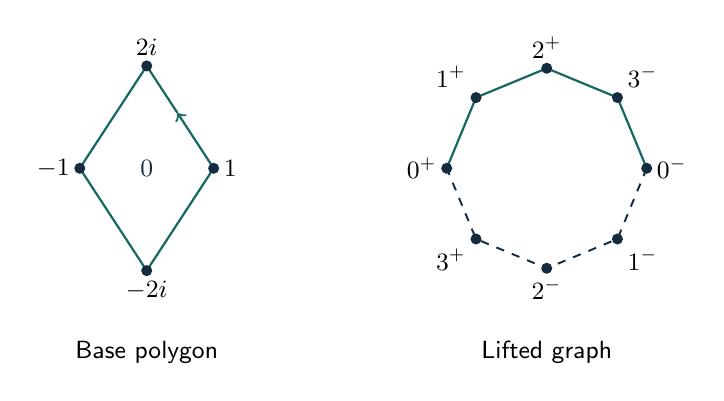
\begin{tikzpicture}[font=\small, line width=.7pt]
\begin{scope}[x=.85cm,y=.65cm,shift={(-2.8,0)}]
\coordinate (a) at (1,0); \coordinate (b) at (0,2); \coordinate (c) at (-1,0); \coordinate (d) at (0,-2);
\draw[accent,thick,->] (a) -- (.46,1.08); \draw[accent,thick] (.46,1.08) -- (b) -- (c) -- (d) -- (a);
\foreach \p in {a,b,c,d} {\fill[ink] (\p) circle(2pt);}
\node[right] at (a) {$1$}; \node[above] at (b) {$2i$};
\node[left] at (c) {$-1$}; \node[below] at (d) {$-2i$};
\node[ink] at (0,0) {$0$};
\node[font=\small\sffamily] at (0,-3.6) {Base polygon};
\end{scope}
\begin{scope}[shift={(2.7,0)}]
\foreach \k in {0,...,7} {\coordinate (v\k) at ({180-45*\k}:1.27);}
\draw[accent,thick] (v0)--(v1)--(v2)--(v3)--(v4);
\draw[ink,dashed] (v4)--(v5)--(v6)--(v7)--(v0);
\foreach \k in {0,...,7} {\fill[ink] (v\k) circle(2pt);}
\node[left] at (v0) {$0^+$}; \node[above left] at (v1) {$1^+$};
\node[above] at (v2) {$2^+$}; \node[above right] at (v3) {$3^-$};
\node[right] at (v4) {$0^-$}; \node[below right] at (v5) {$1^-$};
\node[below] at (v6) {$2^-$}; \node[below left] at (v7) {$3^+$};
\node[font=\small\sffamily] at (0,-2.34) {Lifted graph};
\end{scope}
\end{tikzpicture}
\caption{One counterclockwise traversal of the base polygon lifts to the solid path from $0^+$ to $0^-$. Here $v^{\pm}$ denotes the address $(v,\pm1)$. A second traversal follows the dashed path back to $0^+$.}\label{fig:lift}
\end{figure}


\section{Formalization ledger and remaining questions}\label{sec:formalization}
The canonical deep endpoint in this report is a Lean term of type \texttt{Prf PRAAx} for the translated arithmetic formula. Kernel checking a theorem about Lean finite sets or rational numbers is also useful: it tests the mathematical argument, while leaving the translation to the arithmetic proof system as a separate task. The files below compile without proof holes. Each works at the level indicated.

\begin{center}\small
\begin{tabular}{@{}>{\raggedright\arraybackslash}p{.31\linewidth}>{\raggedright\arraybackslash}p{.63\linewidth}@{}}
\toprule
\textbf{Checked file} & \textbf{Conclusion and scope}\\
\midrule
\texttt{lean/Completion.lean} & A rational distance estimate proving that changing the input name preserves the extension, including its explicit service precision.\\[4pt]
\texttt{lean/Closure.lean} & Finset saturation at $N$, leastness, and exclusion by a cut. For externally given rules and local sequents, \texttt{System.replay} yields an actual ordinary iPRA derivation.\\[4pt]
\texttt{lean/Quotient.lean};\newline\texttt{StableQuotient.lean} & The term-family test for identical transitions; coarseness at a fixed refinement round and lifting through all rounds for the semantic operator.\\[4pt]
\texttt{Merge.lean}; \texttt{Finality.lean} & Native graph, cocone and representable lemmas. \texttt{PathDerivation.lean} compiles fixed-path and merge witnesses into actual iPRA sequents.\\[4pt]
\texttt{NervePolarity.lean};\newline\texttt{NerveTransfer.lean};\newline\texttt{ElementaryCollapse.lean} & A closed iPRA incidence sequent, barycentric collapse identities, and native filtered elimination, cycle lifting, and boundary reflection under the interface in Section~\ref{sec:nerve}.\\[4pt]
\texttt{Secant.lean};\newline\texttt{ContourRibbon.lean} & Native rational derivative comparison and cancellation of the triangulated strip. The full Cauchy and Laurent estimates are human proofs.\\
\bottomrule
\end{tabular}
\end{center}

\paragraph{A deep endpoint for completion.}
Fix symbols for the two validity bits, rational distances, $a,b,E,\mu$. Code each $B_X$ as a pair of outer universal numerical quantifiers with a denominator-cleared comparison. Define $e_n$ by the rational pair $(1,2^n)$; implement $s,L,j$ by bounded integer maximum and composition. For fixed $n,m$ specialize name coherence at exactly the indices in Theorem~\ref{th:completion}, apply the triangle and rational order derivations, then universally close. For the rational gap step, if a positive rational difference is $u/v$ with $u\ge1$, then $2^{-(v+3)}<1/(4v)$ for $v\ge1$ by the elementary induction $2^v\ge v+1$. This gives a numerical index defeating the proposed strict gap without a real-order decision. Composition uses two eliminations of the universal contracts and numerical substitution, so its program parameters remain external throughout.

\paragraph{A concrete next layer for the cyclic calculus.}
Here is a specification for the uniform deep file that remains to be written. Its free numerical parameters are packed into $p=(N,M,(h_i,B_i)_{i<M})$; $W(p)$ checks its lengths and ranges. Define
\[
 \operatorname{en}(i,X)=\prod_{b<N}(1-[b\in B_i](1-[b\in X])),\qquad
 T(X)_a=\max\bigl([a\in X],\ \max_{i<M}[h_i=a]\operatorname{en}(i,X)\bigr).
\]
The outer mask is $\sum_{a<N}2^a T(X)_a$. Define $X(p,j)$ by PR from zero using this expression. Define $\mathsf{pc}(p,a,d)$ by checking length, distinctness, every rule-head pair, its earlier premises and the last head. Define $\mathsf{cut}(p,a,C)$ by the three tests $C<2^N$, $a\notin C$, $T(C)=C$. Let $P(p,a)$ read the table of first rounds and producers and encode the prefix from Theorem~\ref{th:closure}; let $L(p)=X(p,N)$. For $W(p)$ and $a<N$ the target is the universal closure of
\[
 \bigl([a\in L]=1\to\mathsf{pc}(p,a,P(p,a))=1\bigr)
 \ \land\ 
 \bigl([a\in L]=0\to\mathsf{cut}(p,a,L)=1\bigr)
\]
together with $\mathsf{pc}(p,a,d)=1\to\mathsf{cut}(p,a,C)=0$ for arbitrary $d,C$. These formulas do not call an internal interpreter for Lean proofs.

Build the PR symbols from \texttt{PR.comp} and \texttt{PR.prec}. Reuse bounded sums, bit extraction by division with remainder, and \src{Derivations/Lean/IPRADerivations/Foundations/BoundedSyntax.lean}{bounded reflection}. Prove bit replacement and the first-new-bit counting inequality by induction over a prefix of $[N]$. Use Theorem~\ref{th:closure}'s stationary-or-cardinality invariant (or instantiate the repository's \src{Derivations/Lean/IPRADerivations/Foundations/BoundedFixpoint.lean}{bounded fixed-point ascent}). Extend that invariant with the bounded test that each stored birth uses a rule whose premises have earlier nonzero births, and an entry has birth zero iff its current bit is zero. The prefix sorted by birth can be emitted by a double loop over round and address; use $N$ as the bound on its output length. Induct over a checked proof prefix to exclude a simultaneous cut. For refinement, encode a partition by $N$ canonical colour numbers below $N$, a class-union by an $N$-bit mask, and each family term by the image mask of its premises. Bounded reflection applies even to the semantic stability test quantifying over masks $<2^N$. During iteration fix an arbitrary candidate stable refinement $Q$; the invariant that $Q$ refines the current partition is a bounded implication on pairs of addresses. These are direct single-induction targets for the PR formulas behind the native proofs.

\paragraph{From two sheets to arithmetic.}
For the graph of Section~\ref{sec:monodromy}, write $\mathsf{sgn}(v,w)$ as the signed rational inner-product comparison, check each input numerator is separated from zero after clearing denominators, and use $2v+j$ as the address for sign bit $j$. The arithmetic path checker updates $(v,j)$ by an oriented edge and exclusive-or with its negative-label bit. Its prefix invariant is the product formula for the sign of the lifted endpoint. The finite decision theorem now follows from the closure target and the graph-to-path converse. For the analytic adapter, implement dyadic bisection with invariant $l^2\le x\le u^2$, $0\le l\le u$ and the stated interval width. Register the primitive estimates in Lemma~\ref{lem:sqrt-edge}, then derive the mesh argument by an induction whose Boolean invariant compares the computable sign bits. This supplies all data for a complete formalization of the example. This archive includes its finite executable calculation.

\paragraph{Repository evidence and relation to earlier work.}
The pinned revision is \href{https://github.com/VladimirReshetnikov/ProveIt/tree/3ee850b4c2d650cf01263823fd5415963747c5d0/Logic/PrimitiveRecursiveArithmetic}{\texttt{3ee850b4c2d6}}. The \src{README.md}{directory guide} distinguishes delivered packets from kernel-checked derivations. The \src{Derivations/FINITE-DEMAND-CLAIMS.md}{finite-demand audit} already records checked bounded reflection, backward demand, and parameter-changing recursion. The \src{Derivations/FIBER-CLAIMS.md}{FIBER audit} and \src{Derivations/Lean/IPRADerivations/Foundations/TwoCoordinateDemandClosure.lean}{two-coordinate closure} describe the residual cyclic-certificate problem. Our finite positive production result treats one fragment of it. The \src{Derivations/Lean/IPRADerivations/Foundations/FiniteCoequalizer.lean}{coequalizer module}, \src{docs/proofs/topology/ipra_topology_framework_2026-11-15/paper/sections/12_limits.tex}{topology research questions}, and \src{docs/proofs/analysis/cauchy_residue_ipra/report.tex}{Cauchy--residue manuscript} give the specific boundaries addressed in the three applications. Classical finality and nerve comparisons are established mathematics. The claims here concern explicit arithmetic hypotheses, constructions, witnesses and derivations.

\paragraph{Further research questions.}
\begin{enumerate}
\item Can the positive production calculus be integrated with the FIBER compiler so that a finite bound on all jointly used evidence values is itself inferred for additional cyclic source constructs? An informative test case is a cycle whose individual requests are bounded but whose successful witnesses must agree on a long common partial map.
\item Can the geometric construction of Section~\ref{sec:collapse-nerve} be extended beyond collapsible intersections using PR-bounded expansions followed by collapses? The homological test already handles a wider class over $\mathbb F_2$, where it produces a linear contraction. A geometric extension would have to produce actual homotopies on the represented spaces.
\item Can rational proxy holes and a valid global filling be generated from a more economical input, such as an effective polygonal domain with an explicit collar radius? Section~\ref{sec:named-residue} supplies centre translation with quantified margins; producing those margins from mere negative information about a singular set remains a separate problem.
\end{enumerate}

\end{document}
